%% This is the ctufit-thesis example file. It is used to produce theses
%% for submission to Czech Technical University, Faculty of Information Technology.
%%
%% Get the newest version from
%% https://gitlab.fit.cvut.cz/theses-templates/FITthesis-LaTeX
%%
%%
%% Copyright 2021, Eliska Sestakova and Ondrej Guth
%%
%% This work may be distributed and/or modified under the
%% conditions of the LaTeX Project Public Licenese, either version 1.3
%% of this license or (at your option) any later version.
%% The latest version of this license is in
%%  https://www.latex-project.org/lppl.txt
%% and version 1.3 or later is part of all distributions of LaTeX
%% version 2005/12/01 or later.
%%
%% This work has the LPPL maintenance status `maintained'.
%%
%% The current maintainer of this work is Ondrej Guth.
%% Contact ondrej.guth@fit.cvut.cz for bug reports.
%% Alternatively, submit bug reports into the tracker at
%% https://gitlab.fit.cvut.cz/theses-templates/FITthesis-LaTeX/issues
%%
%%

%%%%%%%%%%%%%%%%%%%%%%%%%%%%%%%%%%%%%%%%%
% CLASS OPTIONS
% language: czech/english/slovak
% thesis type: bachelor/master/dissertation
% colour: bw for black&white OR no option for default colour scheme
%%%%%%%%%%%%%%%%%%%%%%%%%%%%%%%%%%%%%%%%%
\documentclass[english,master,unicode]{ctufit-thesis}

%%%%%%%%%%%%%%%%%%%%%%%%%%%%%%%%%%
% FILL IN THIS INFORMATION
%%%%%%%%%%%%%%%%%%%%%%%%%%%%%%%%%%
\ctufittitle{Multiple target tracking with external information} % replace with the title of your thesis
\ctufitauthorfull{Bc. Andrey Babushkin} % replace with your full name (first name(s) and then family name(s) / surname(s)) including academic degrees
\ctufitauthorsurnames{Babushkin} % replace with your surname(s) / family name(s)
\ctufitauthorgivennames{Andrey} % replace with your first name(s) / given name(s)
\ctufitsupervisor{doc.\,Ing.\,Kamil Dedecius,\,Ph.D.} % replace with name of your supervisor/advisor (include academic degrees)
\ctufitdepartment{Department of Applied Mathematics} % replace with the department of your defence
\ctufityear{2023} % replace with the year of your defence
\ctufitdeclarationplace{Prague} % replace with the place where you sign the declaration
\ctufitdeclarationdate{\today} % replace with the date of signature of the declaration
\ctufitabstractCZE{Tato práce se zaměřuje na problém sledování více cílů v prostředí s vysokým množstvím rušení a nejistotou ohledně počtu sledovaných objektů pomocí Bayesovské inference. V této práci se hlavně zaměřujeme na populární Gaussian mixture probability hypothesis density (GM-PHD) filtr a představujeme techniku, jak zahrnout dodatečné informace pro případy, kdy senzor nedokáže detekovat sledované objekty z důvodu fyzických nebo prostředkových omezení. Poskytujeme veškeré potřebné teoretické pozadí od základů teorie pravděpodobnosti až po diskusi o různých metodách sledování více cílů a představení rámce Finite Set Statistics (FISST). Dále zahrnujeme rozsáhlé měření výkonnosti a analýzu výsledků, kde ukazujeme, že navržená technika fúze výrazně zlepšuje sledovací výsledky. Nakonec diskutujeme omezení filtru a navrhujeme možné způsoby, jak je překonat.
}
\ctufitabstractENG{The thesis focuses on the multi-target tracking problem in cluttered environments with the uncertainty on the number of targets and using Bayesian inference. In this work, we mainly focus on the popular Gaussian mixture probability hypothesis density (GM-PHD) filter and introduce a technique to include additional information for cases when a sensor fails to detect targets due to environmental or physical limitations. We provide all required theoretical background from the basics of probability theory to the discussion of various multi-target tracking methods and the introduction of the Finite Set Statistics (FISST) framework. We also conclude with an extensive performance measurement and analysis of results, where we demonstrate that the proposed fusion technique significantly improves tracking results. Finally, we discuss the limitations of the filter and propose possible measures to overcome them.
}
\ctufitkeywordsCZE{Bayesovské filtrování, sledování více cílů, náhodné množiny, gaussian mixture probability density filtr, fúze externích informací}
\ctufitkeywordsENG{Bayesian filtering, multi-target tracking, random finite sets, Gaussian Mixture Probability Density filter, external information fusion
}
%%%%%%%%%%%%%%%%%%%%%%%%%%%%%%%%%%
% END FILL IN
%%%%%%%%%%%%%%%%%%%%%%%%%%%%%%%%%%

%%%%%%%%%%%%%%%%%%%%%%%%%%%%%%%%%%
% CUSTOMIZATION of this template
% Skip this part or alter it if you know what you are doing.
%%%%%%%%%%%%%%%%%%%%%%%%%%%%%%%%%%

\RequirePackage{iftex}[2020/03/06]
\iftutex % XeLaTeX and LuaLaTeX
    \RequirePackage{ellipsis}[2020/05/22] %ellipsis workaround for XeLaTeX
\else
    \RequirePackage[utf8]{inputenc}[2018/08/11] %this file encoding
    \RequirePackage{lmodern}[2009/10/30] % vector flavor of Computer Modern font
\fi

% hyperlinks
\RequirePackage[pdfpagelayout=TwoPageRight,colorlinks=false,allcolors=decoration,pdfborder={0 0 0.1}]{hyperref}[2020-05-15]

% uncomment the following to hide all hyperlinks
% \RequirePackage[pdfpagelayout=TwoPageRight,hidelinks]{hyperref}[2020-05-15]

\RequirePackage{pdfpages}[2020/01/28]

\setcounter{secnumdepth}{4} % numbering sections; 4: subsubsection

%%%%%%%%%%%%%%%%%%%%%%%%%%%%%%%%%%
% CUSTOMIZATION of this template END
%%%%%%%%%%%%%%%%%%%%%%%%%%%%%%%%%%


%%%%%%%%%%%%%%%%%%%%%%
% DEMO CONTENTS SETTINGS
% You may choose to modify this part.
%%%%%%%%%%%%%%%%%%%%%%
\usepackage{dirtree}
\usepackage{lipsum,tikz}
\usepackage{csquotes}
\usepackage[style=iso-numeric]{biblatex}
\addbibresource{text/references.bib}
\usepackage{listings} % typesetting of sources
\usepackage{caption}
\usepackage{subcaption}  % subfigures
\usepackage{mathrsfs}  % mathscr
\usepackage{todonotes}  % TODOs that are not later lost
\usepackage{epigraph}  % nice quotes
\usepackage{algorithm}  % algorithms
\usepackage{algpseudocode}  % pseudocode elements
% \usepackage{minted} % typesetting of sources

%theorems, definitions, etc.
\theoremstyle{plain}
\newtheorem{theorem}{Theorem}
\newtheorem{lemma}[theorem]{Lemma}
\newtheorem{corollary}[theorem]{Corollary}
\newtheorem{proposition}[theorem]{Proposition}
\newtheorem{definition}[theorem]{Definition}
\theoremstyle{definition}
\newtheorem{example}[theorem]{Example}
\theoremstyle{remark}
\newtheorem{note}[theorem]{Note}
\newtheorem*{note*}{Note}
\newtheorem{remark}[theorem]{Remark}
\newtheorem*{remark*}{Remark}
\numberwithin{theorem}{chapter}
%theorems, definitions, etc. END
%%%%%%%%%%%%%%%%%%%%%%
% DEMO CONTENTS SETTINGS END
%%%%%%%%%%%%%%%%%%%%%%

\begin{document} 
\frontmatter\frontmatterinit % do not remove these two commands


\includepdf[pages={1-}]{assignment-include.pdf} % replace that file with your thesis assignment provided by study office

\thispagestyle{empty}\cleardoublepage\maketitle % do not remove these three commands

\imprintpage % do not remove this command

\tableofcontents % do not remove this command
%%%%%%%%%%%%%%%%%%%%%%
% list of other contents: figures, tables, code listings, algorithms, etc.
% add/remove commands accordingly
%%%%%%%%%%%%%%%%%%%%%%
\listoffigures % list of figures
\begingroup
\let\clearpage\relax
\listoftables % list of tables
\lstlistoflistings % list of source code listings generated by the listings package
% \listoflistings % list of source code listings generated by the minted package
\endgroup
%%%%%%%%%%%%%%%%%%%%%%
% list of other contents END
%%%%%%%%%%%%%%%%%%%%%%

\include{text/acknowledment}
%%%%%%%%%%%%%%%%%%%
% DECLARATION
% FILL IN / MODIFY
%%%%%%%%%%%%%%%%%%%
% INSTRUCTIONS
% ENG: choose one of approved texts of the declaration. DO NOT CREATE YOUR OWN. Find the approved texts at https://courses.fit.cvut.cz/SFE/download/index.html#_documents (document Declaration for FT in English)
% CZE/SLO: Vyberte jedno z fakultou schvalenych prohlaseni. NEVKLADEJTE VLASTNI TEXT. Schvalena prohlaseni najdete zde: https://courses.fit.cvut.cz/SZZ/dokumenty/index.html#_dokumenty (prohlášení do ZP)
\begin{declarationpage}
I hereby declare that the presented thesis is my own work and that I have cited all sources of information in accordance with the Guideline for adhering to ethical principles when elaborating an academic final thesis.

I acknowledge that my thesis is subject to the rights and obligations stipulated by the Act No. 121/2000 Coll., the Copyright Act, as amended, in particular that the Czech Technical University in Prague has the right to conclude a license agreement on the utilization of this thesis as a school work under the provisions of Article 60 (1) of the Act.
\end{declarationpage}
%%%%%%%%%%%%%%%%%%%
% DECLARATION END
%%%%%%%%%%%%%%%%%%%

\printabstractpage % do not remove this command
%%%%%%%%%%%%%%%%%%%
% SUMMARY
% FILL IN / MODIFY
% OR REMOVE ENTIRELY (upon agreement with your supervisor)
% (appropriate to remove in most theses)
%%%%%%%%%%%%%%%%%%%
\begin{summarypage}
\section*{Summary section}

\lipsum[1][1-8]

\section*{Summary section}

\lipsum[2][1-6]

\section*{Summary section}

\lipsum[3]

\section*{Summary section}

\lipsum[2]

\section*{Summary section}

\lipsum[1][1-8] Lorem lorem lorem.
\end{summarypage}
%%%%%%%%%%%%%%%%%%%
% SUMMARY END
%%%%%%%%%%%%%%%%%%%

\chapter{List of Acronyms}%%%%%%%%%%%%%%%%%%%
% ABBREVIATIONS
% FILL IN / MODIFY
% OR REMOVE ENTIRELY
% List the abbreviations in lexicography order.
%%%%%%%%%%%%%%%%%%%
\chapter{List of Acronyms}

\begin{tabular}{rl}
CV & Constant Velocity \\
EKF & Extended Kalman filter \\
FISST & Finite Set Statistics \\
FoV & Field of view \\
GM & Gaussian mixture \\
HO-MHT & Hypothesis-oriented Multiple Hypothesis Tracker \\
JPDA & Joint Probabilistic Data Association \\
KF & Kalman filter \\
MAP & Maximum a posteriori \\
MHT & Multiple Hypothesis Tracker \\
MLE & Maximum Likelihood Estimator \\
MMSE & Minimum Mean Square Error \\
MTT & Multitarget tracking \\
PDA & Probabilistic Data Association \\
PHD & Probability hypothesis density \\
PPP & Poisson Point Process \\
RFS & Random Finite Set \\
TO-MHT & Track-oriented Multiple Hypothesis Tracker \\
UKF & Unscented Kalman Filter \\
\end{tabular}
%%%%%%%%%%%%%%%%%%%
% ABBREVIATIONS END
%%%%%%%%%%%%%%%%%%%


%%%%%%%%%%%%%%%%%%%
% THE THESIS
% MODIFY ANYTHING BELOW THIS LINE
%%%%%%%%%%%%%%%%%%%

%%%%%%%%%%%%%%%%%%%%%%%%%%%%%%%%%%%%%%%%%%
% Commands
%%%%%%%%%%%%%%%%%%%%%%%%%%%%%%%%%%%%%%%%%%
\newcommand{\varat}[2]{\relax\ifmmode{#1}_{#2}\else ${#1}_{#2}$\fi}
\newcommand{\vecat}[2]{\relax\ifmmode\mathbf{#1}_{#2}\else $\mathbf{#1}_{#2}$\fi}
\newcommand{\svecat}[3]{\relax\ifmmode\vecat{#1}{#2}^{#3}\else $\vecat{#1}{#2}^{#3}$\fi}
\renewcommand{\Pr}[1]{\operatorname{Pr}\{#1\}}

\graphicspath{figures}
\mainmatter\mainmatterinit % do not remove these two commands

%%%%%%%%%%%%%%%%%%%%%%%%%%%%%%%%%%%%%%%%%%
% Introduction
%%%%%%%%%%%%%%%%%%%%%%%%%%%%%%%%%%%%%%%%%%
\addcontentsline{toc}{chapter}{Introduction}\markboth{Introduction}{Introduction}
\setcounter{page}{1}

\chapter*{Introduction}Object tracking is a critical problem in signal processing and computer vision. The primary goal of tracking algorithms is to estimate the states of moving targets based on a sequence of sensor measurements in environments with a high degree of uncertainty. Different domains of the problem require different approaches to target tracking. In this work, we provide an overview of the existing areas of target tracking and introduce the scope of this study.

Tracking algorithms can be categorized based on the number of targets they track, whether it is a fixed or known number of targets, or a variable and unknown number of targets. When the number of targets in the tracking area is greater than one, we refer to it as multi-target tracking (MTT). Object tracking is widely used in various fields, including robotics, autonomous vehicles, surveillance, and medical imaging. With the recent emergence of deep learning algorithms, there has been renewed interest in MTT, and many new deep learning-based approaches have been proposed. However, the learned model's predictive power is questionable, as these approaches estimate the internal object dynamics using complex non-linear models, while the Bayesian approach assumes fixed known model that are specified manually according to some prior knowledge, for instance, physical laws. In this study, we focus on MTT using Bayesian inference, the statistical approach based on recursive updates of the target posterior distribution using a set of measurements.

Bayesian algorithms are classified based on the results they achieve \cite[11]{sarkkaBayesianFilteringSmoothing2013}. The first type of algorithms is Bayesian smoothers, which remove the noise of states based on past and future measurements, i.e., they smooth the signal. The other type is Bayesian predictors, which predict the future state of a target more than one step ahead based on past measurements. The last type is Bayesian filters, which predict the current state of a target based on measurements up to the moment of the predicted state. The Kalman filter, the fundamental algorithm for many modern and sophisticated tracking methods, is an example of Bayesian filters. This study focuses on Bayesian filters, and we cover the Kalman filter in detail.

Algorithms can also be separated based on the type of sensor and measurements used. There are several sets of algorithms available to address specific problems depending on the sensors used. For instance, point object tracking is used when the sensor generates one measurement per object, such as a radar or a camera with an object recognition algorithm. When lidars are used, one target generates a set of measurements, and this is referred to as extended object tracking \cite{granstromExtendedObjectTracking2017}. In surveillance, especially when tracking people, group object tracking algorithms are used to estimate groups of individuals rather than every individual separately \cite{salmondGroupExtendedObject1999}. Additionally, tracking with multipath propagation refers to scenarios where a sensor receives more than one detection caused by the multipath phenomenon or multiple reflections from surrounding objects of the same signal \cite{bar-shalomTrackingLowElevation1994}. Finally, tracking with unresolved targets occurs when several targets produce only one measurement \cite{angleMultipleTargetTracking2021}. In this study, we focus on point object tracking, assuming that one target produces at most one measurement, and each measurement can be generated by at most one target.

This study aims to enhance the performance of the Gaussian Mixture probability hypothesis density (GM-PHD) filter, a popular Bayesian filter for multi-target tracking (MTT), by proposing a novel approach to incorporate external information. Specifically, we provide a detailed description of the GM-PHD filter and its internals, and demonstrate through an example how the filter may fail under environmental limitations. We then introduce our proposed method for integrating external information and analyze its impact on the filter's performance. Finally, we evaluate the filter's strengths and weaknesses in various scenarios and discuss the significance of our contribution in improving the accuracy and robustness of the GM-PHD filter for MTT.

\section*{Motivation}% Motivation of this work
% main questions and goals

\section*{Related works}% Previous research on object tracking
% different Bayesian filters, GM-PHD, etc.

\section*{Contribution of this work}% Contribution of the work
\section*{Structure}The thesis is structured as follows. Chapter 1 provides the theoretical background necessary for understanding the rest of the thesis, including the introduction of probability theory and probability distributions and the Bayes' rule. Next, we present the Bayesian inference framework, which is the basis for the general Bayes filter, a recursive algorithm for state estimation. Finally, we present the concepts of state-space models and the Kalman filter.

Chapter 2 is dedicated to multi-target tracking. It starts with an overview of target tracking methods, followed by an introduction to Random Finite Sets (RFS). The chapter then describes the PHD filter and the PHD function. Next, we give a PHD filter formal definition, and then observe the Gaussian Mixture PHD filter. The chapter concludes with a discussion of track maintenance, the GM-PHD recursion, and ends with the framework for external information fusion.

Chapter 3 describes the implementation and testing methodology of the GM-PHD filter. We then introduce several metrics that are used to measure the performance of multi-target tracking algorithms, then we describe four testing scenarios. The final section on parameters testing and methodology explains how the tests were conducted and how the results were analyzed.

Chapter 4 analyzes the results of the tests conducted in Chapter 3. This chapter includes sections on test results for each scenario and a discussion of the results, where a comprehensive analysis of the filter strengths and weaknesses is provided.

The final Chapter 5 concludes this work by summarizing the main contributions of the thesis and highlighting areas for future research.


%%%%%%%%%%%%%%%%%%%%%%%%%%%%%%%%%%%%%%%%%%
% Theoretical background
%%%%%%%%%%%%%%%%%%%%%%%%%%%%%%%%%%%%%%%%%%
\chapter{Theoretical background}\label{ch:theory}
    \section{Probability theory foundations}\label{sec:prob-foundations}
        When we are dealing with probability of an event, we assume that there is a possibility
of that event occurring and we measure it using a number between 0 and 1 or a percentage
between 0\% and 100\%. In other words, we use the probability theory framework to assign
numerical values to arbitrary events. This section covers several fundamental concepts of
probability theory, which serve as the basis for this work.

The \textit{event}, which we formally denote as $E$, comes from some space of all possible
events, the \textit{outcome space} $\Omega$. We also denote the \textit{probability} of the
event $E$ as $\Pr{E}$. This probability is a real non-negative number,
that is $\Pr{E} \in \mathbb{R}, \Pr{E} \geq 0$. The outcome
space covers all possible events, that is $\Pr{\Omega} = 1$. It then follows
that the probability of disjoint events from the outcome space $\Omega$ is the sum of
probabilities of these events, that is for
$E_1, \ldots, E_n \in \Omega, \Pr{\bigcup_{i=1}^n E_i} = \sum_{i=1}^n \Pr{E_i}$.

We have defined three main axioms of probability theory. In addition to these axioms, several
crucial concepts illustrate the relationship between events. Given two events, $E_1$ and $E_2$,
the \textit{conditional probability} of $E_1$ given $E_2$ is defined as

$$
\Pr{E_1 \mid E_2} = \frac{\Pr{E_1 \cap E_2}}{\Pr{E_2}}.
$$

If the events are \textit{independent} of each other, the probability of them occurring
simultaneously is given by

$$
\Pr{E_1 \cap E_2} = \Pr{E_1}\Pr{E_2}.
$$

These relationships allow us to define the \textit{law of total probability}
\cite[31]{zwillingerCRCStandardProbability2000}, which is a key component of Bayes' rule.
Let $A$ be an event, $A \int \Omega$, and $\{B_n : n = 1, 2, \ldots\}$ be a countable
partition of the space $\Omega$. Then, we have:

$$
\Pr{A} = \sum_n \Pr{A \mid B_n} \Pr{B_n}.
$$

Now, we can deduce the following rule:

\begin{definition}[Bayes' rule]
Let $A$ and $B$ be two events from the outcome space $\Omega$. Then the following applies:

$$
\Pr{A \mid B} = \frac{\Pr{B \mid A}}{\Pr{B}}
    = \frac{\Pr{B \mid A}}{\sum_n \Pr{B \mid A_n}\Pr{A_n}}.
$$
\end{definition}

Bayes' rule plays a crucial role in Bayesian inference and serves as the basis for
Bayesian filters, including the PHD filter.

        \subsection{Probability distributions}\label{sec:prob-distributions}
            Events and their probabilities are not sufficient for our purposes;
we need a framework that allows us to obtain a formal, general description of a set
of events from some outcome space. Specifically, we need an abstraction around events,
which is some function that maps the outcome space $\Omega$ to some other space,
typically $\mathbb{R}$ (but not necessarily). This abstraction is called a
\textit{random variable} and one outcome of it is called a \textit{realization}.

\begin{definition}[Random variable and its realization]
    Let $\Omega$ be a set of possible events, $\omega \in \Omega$ is some event,
    and $\mathbb{O}$ be another space. A function $X: \Omega \rightarrow \mathbb{O}$
    is called a random variable and $x = X(\omega)$ is called a realization of $X$.
\end{definition}

The above definition provides a general framework for understanding random variables.
However, for the purposes of Bayesian statistics, we will simplify the discussion by
focusing on scalar, continuous-valued random variables, represented
by $\mathbb{O} = \mathbb{R}$. In practice, it is often impractical to calculate the
probability of every possible event from the outcome space $\Omega$, especially for
continuous random variables with uncountably infinite outcomes. Instead, it may suffice
to work with intervals on the outcome space and their probabilities. We call such a
probability distribution a \textit{cumulative distribution function (cdf)} of $X$,
and the first-order derivative of the cdf is called a \textit{probability density
function (pdf)}.\footnote{
    For discrete random variables, the corresponding distribution function is
    called a \textit{probability mass function (pmf)}.
}

\begin{definition}[Cumulative distribution function (cdf)]
    Given a scalar real-valued random variable $X \in \mathbb{R}$ and $x$ as a
    realization of $X$, we define the probability $\Pr{X \in (-\infty, x)} = \Pr{X < x}$
    as the cumulative distribution function of random variable $X$ and denote it as $P(x)$.
\end{definition}

\begin{definition}[Probability density function (pdf)]
    The probability density function $p(x)$ of a scalar real-valued random variable $X$
    is defined as:
    $$
    p(x) = \frac{\partial P(x)}{\partial x}.
    $$
\end{definition}

Probability distributions are fundamental in Bayesian statistics and provide a way
to model and analyze the behavior of random variables. In the next section,
we will discuss some common probability distributions used in Bayesian filters,
including the Gaussian distribution and the Poisson distribution.

Probability distributions are fundamental in Bayesian statistics and provide a way
to model and analyze the behavior of random variables. Cdfs and pdfs (as well as pmfs
for discrete cases) are used to specify the probability distribution of a random
variable, providing a formal description of the relationship
between events and probabilities. In addition to this formal description, we also
need to know several statistical properties of probability distributions to fully
understand their behavior. Two main properties of probability distributions are
the expected value, $E[X]$, and the variance, $\operatorname{Var}[X]$:

$$
\begin{aligned}
E[X]&=\int_{-\infty}^{\infty} x p(x) d x, \\
\operatorname{Var}[X]
    &= E\left[(X-E[X])^2\right]
    =\int_{-\infty}^{\infty}(x-E[X])^2 p(x) d x.
\end{aligned}
$$

The expected value, or the first moment, represents the most probable value of
a random variable. The variance, or the second central moment, is a measure of the
variability of a random variable and is often denoted as $\operatorname{Var}[X] = \sigma^2$.
Furthermore, we often study the relationship between two random variables, say $X$ and
$Y$, and measure their joint variability, which we call a \textit{covariance}:

$$
\operatorname{Cov}[X, Y]
    = E\left[(X-E[X])(Y-E[Y])\right]
    =\int_{-\infty}^{\infty}(x-E[X])(y-E[Y]) p(x, y) d x d x.
$$

For vector-valued random variables, that is $X, Y \in \mathbb{R}^k$ and $\mathbf{x}$
is the realization of $X$, the formulas are the following. It is worth noting that
the covariance in the vector case becomes a matrix and is called a \textit{covariance
matrix}:

$$
\begin{aligned}
E[X]
    &=\int_{-\infty}^{\infty} \mathbf{x} p(\mathbf{x}) d \mathbf{x}, \\
\operatorname{Var}(X)
    &= E\left[\left(X-E[X]\right)\left(X-E[X]\right)^\intercal\right]
    \\&=\int_{-\infty}^{\infty}
        \left(\mathbf{x}-E[X]\right)
        \left(\mathbf{x}-E[X]\right)^\intercal
        p(\mathbf{x})
        d \mathbf{x}, \\
\operatorname{Cov}[X, Y]
    &= E\left[\left(X-E[X]\right)\left(Y-E[Y]\right)^\intercal\right]
    \\&=\int_{-\infty}^{\infty}
        \left(\mathbf{x}-E[X]\right)
        \left(\mathbf{y}-E[Y]\right)^\intercal
        p(\mathbf{x}, \mathbf{y})
        d \mathbf{x} d \mathbf{y}.
\end{aligned}
$$

Probability distributions are fundamental in Bayesian statistics and
provide a way to model and analyze the behavior of random variables. For
the purpose of Bayesian filters, some common probability distributions
are particularly useful. In this section, we will discuss some of these
distributions and their main properties. We shall start from discrete
cases and go on to the continuous variables.  % uniform, bernoulli, poisson, gaussian

            \subsubsection{Bernoulli distribution}\label{sec:bernoulli-distribution}
                The Bernoulli distribution is the simplest discrete probability
distribution, and the Bernoulli random variable is binary, with only
two realizations, $0$ or $1$. This distribution is parameterized with 
$r$, the probability of the positive outcome. Its probability mass 
function is given by

$$
p(x) = \begin{cases}
 1 - r, & \text{if } x = 0, \\
     r, & \text{if } x = 1, \\
     0, & \text{otherwise}.
\end{cases}
$$

\begin{figure}
\centering
\begin{subfigure}{.5\textwidth}
  \centering
  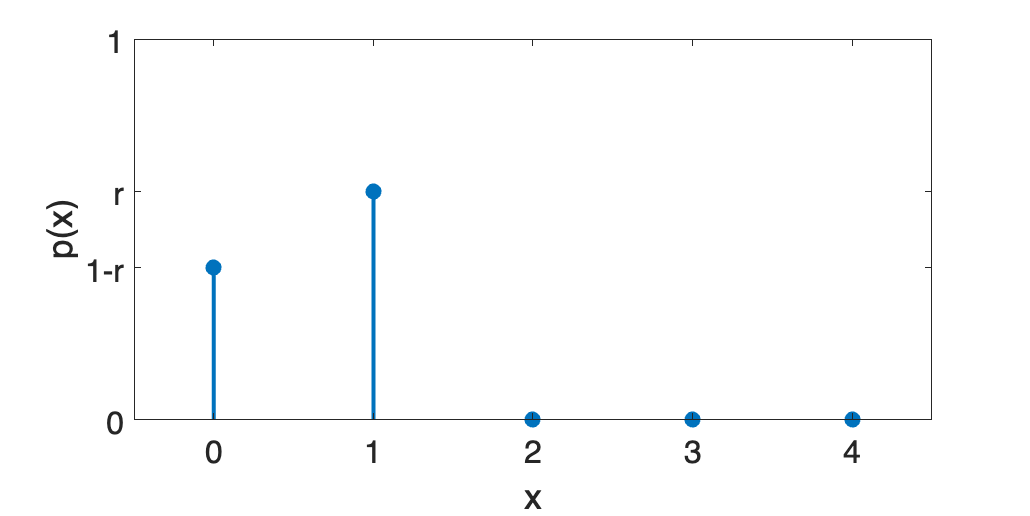
\includegraphics[width=.9\linewidth]{figures/bern.pmf.png}
  \caption{PMF.}
  \label{fig:bern:pmf}
\end{subfigure}\hfill
\begin{subfigure}{.5\textwidth}
  \centering
  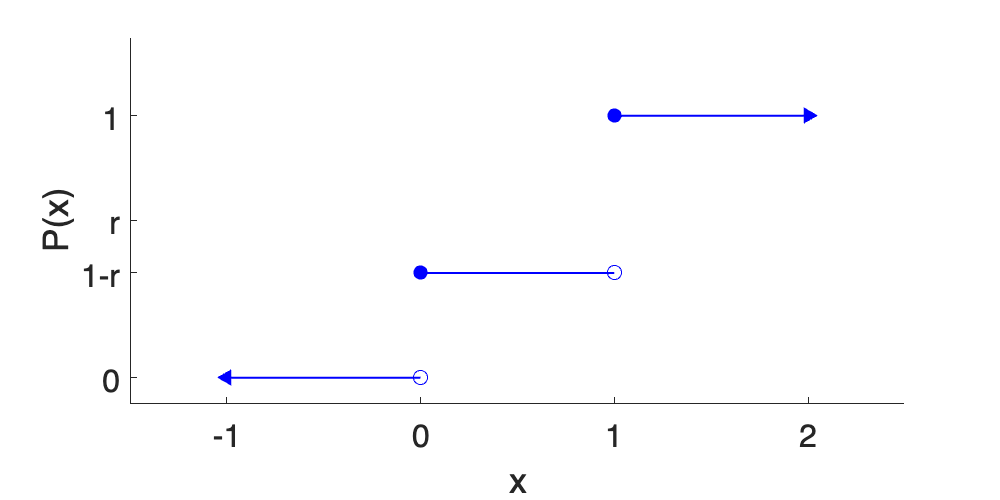
\includegraphics[width=.9\linewidth]{figures/bern.cdf.png}
  \caption{CDF.}
  \label{fig:bern:cdf}
\end{subfigure}
\caption[An example of the Bernoulli distribution.]{Bernoulli distribution.}
\label{fig:bern}
\end{figure}

The pmf and the cdf of the Bernoulli distribution can be seen on Figure \ref{fig:bern}.
We denote this distribution as $p(x) = \operatorname{Bernoulli}(x;r)$.
The expected value and the covariance of a Bernoulli random variable $X$ are

$$
E[X] = r, \qquad \operatorname{Var}[X] = r(1-r).
$$

In object tracking, we use Bernoulli random variables to model the existence of
an object at some time step $k$, which we will discuss in detail in the following
sections.

            \subsubsection{Binomial distribution}\label{sec:binomial-distribution}
                Binomial random variables are the generalization of Bernoulli random variables,
representing the probability of $x$ positive outcomes after $n$ consecutive and
independent trials. This distribution is parameterized by the probability of the
positive outcome in one trial $r$ and the number of trials $n$. Its pmf, as well 
as the expected value and the variance, are given by

\begin{equation}
\begin{aligned}
    p(x) &= \binom{n}{x} r^x (1-r)^{(n-x)}, \\
    E[X] &= nr, \\
    \operatorname{Var}[X] &= nr(1-r).
\end{aligned}
\end{equation}

            \subsubsection{Poisson distribution}\label{sec:poisson-distribution}
                The Poisson distribution is a discrete random distribution that can 
be used as an approximation of the Binomial distribution in cases where 
$n$ tends towards infinity and $r$ tends towards $0$ such that their 
product stays about equal to a parameter $\lambda$, which is the 
parameter of the Poisson distribution and also its expected value and 
variance. The outcome space of a Poisson random variable is 
$\mathbb{N}_0$, that is natural numbers including $0$, and its pmf,
expected value and variance are given by

\begin{align}
    p(x) = \operatorname{Poisson}(x; \lambda) &= \frac{\lambda^x e^{-\lambda}}{x !}, \\
    E[X] = \operatorname{Var}[X] &= \lambda.
\end{align}

The probability mass function and the corresponding cumulative density functions
of the Poisson distribution can be seen in Figure \ref{fig:poisson}.
The Poisson distribution is a critical component of modern multi-object
tracking systems, as it is used to model noise measurements, and some 
systems even use it to model objects that exist but are not visible in
the field of view of a sensor \cite{garcia-fernandezPoissonMultiBernoulliMixture2018}.
The Poisson distribution is the foundation of the so-called Poisson Point
Processes (PPP), which will be discussed later.

\begin{figure}
\centering
\begin{subfigure}{.5\textwidth}
  \centering
  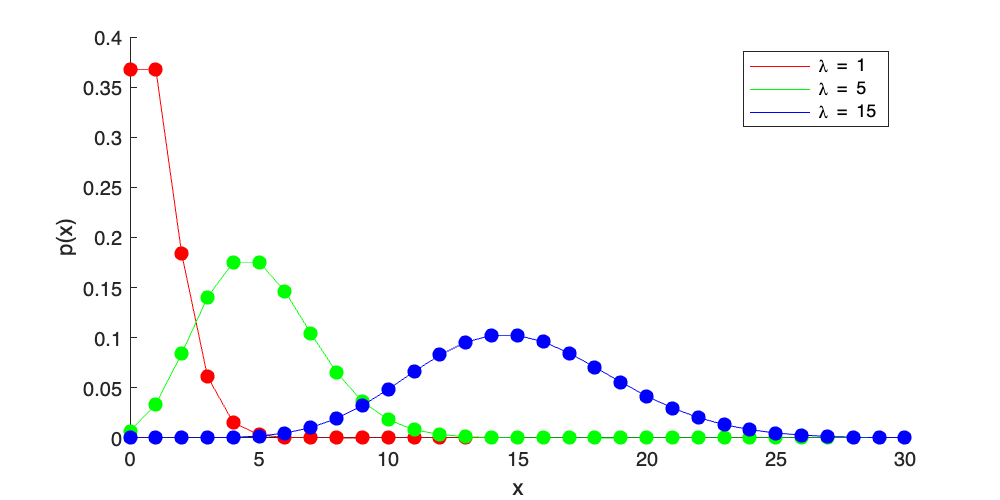
\includegraphics[width=.9\linewidth]{figures/poisson.pmf.png}
  \caption{PMF.}
  \label{fig:poisson:pmf}
\end{subfigure}\hfill
\begin{subfigure}{.5\textwidth}
  \centering
  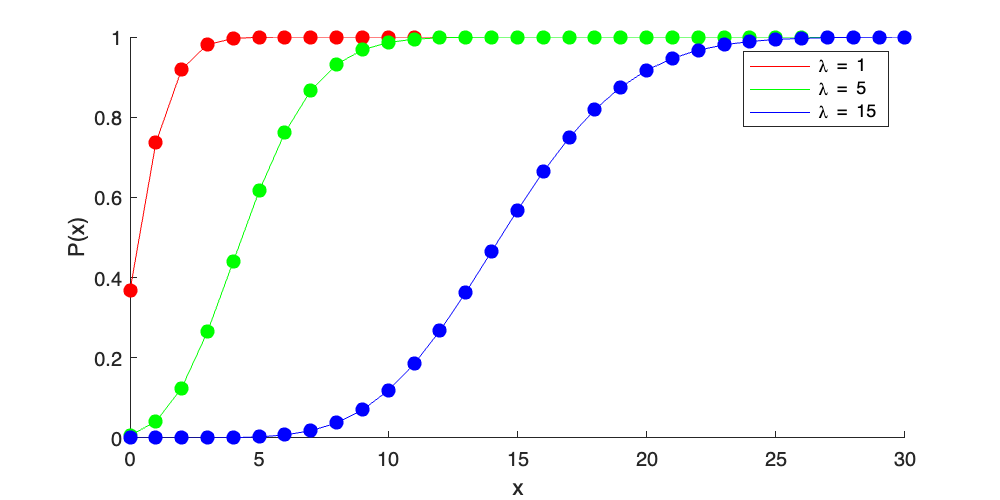
\includegraphics[width=.9\linewidth]{figures/poisson.cdf.png}
  \caption{CDF.}
  \label{fig:poisson:cdf}
\end{subfigure}
\caption[An example of the Bernoulli distribution.]{Poisson distribution.}
\label{fig:poisson}
\end{figure}

            \subsubsection{Uniform distribution}\label{sec:uniform-distribution}
                The uniform distribution is a continuous probability distribution and it
describes such random variables which outcomes on some interval $[a, b]$
are possible with equal probability. This distribution is parameterized by
$a$ and $b$ and its pdf, $E[X]$ and $\operatorname{Var}[X]$ are:

\begin{align}
    p(x)
        =\operatorname{Uniform}(x; [a, b])
        &= \begin{cases}
            \frac{1}{b-a} & \text { if } a \leq x \leq b, \\
            0 & \text { otherwise, }
        \end{cases} \\
    E[X] &= \frac{a + b}{2}, \\
    \operatorname{Var}[X] &= \frac{(b - a)^2}{12}.
\end{align}

The uniform distribution is generally used to represent the uncertainty when
all outcomes are equally possible. In this work, we use the uniform distribution
to model positions of clutter measurements at some time step $k$.

            \subsubsection{Gaussian distribution}\label{sec:gaussian-distribution}
                The Gaussian distribution, also known as the normal distribution, is a 
continuous probability distribution that is widely used in many branches
of statistics, including Bayesian filtering. It is typically used to model
a large number of independent and identically distributed (i.i.d.) random variables.

The Gaussian distribution is characterized by two parameters: the mean 
$\mu$ and the variance $\sigma^2$. Its probability density function (pdf), 
expected value, and variance are given by:

\begin{align}
    p(x)
        =\mathscr{N}\left(x ; \mu, \sigma^2\right)
        &=\frac{1}{\sqrt{2 \pi} \sigma} \exp \left(\frac{(x-\mu)^2}{2 \sigma^2}\right), \\
    E[X] &= \mu, \\
    \operatorname{Var}[X] &= \sigma^2.
\end{align}

In the notation $\mathscr{N}\left(x ; \mu, \sigma^2\right)$, the first 
parameter $x$ means ``evaluated at.''
Despite the cdf of the Gaussian distribution not having a closed-form 
representation, the distribution possesses several desirable properties that 
allow for closed-form solutions in many applications, including object 
tracking. Although it may be too simple to model certain scenarios, it 
represents the approximate average position of objects and their uncertainty 
quite well. This work utilizes mixtures of Gaussians, which will be discussed 
in more detail later.

    \section{Bayesian inference}\label{sec:bayesian-inference}
        % Bayesian inference
    % - [x] Overview of Bayesian inference and its advantages over frequentist methods
    % - [x] Sequential application
% Estimators
    % - [x] MLE and MAP
    % - [x] What is better and why

In statistics, there are two ways to understand the uncertainty. The first one,
called \textit{frequentist}, assumes that the source of uncertainty lays in the
nature of events. If we modeled a random process following this approach, we 
would calculate parameters of the model using their maximum likelihood 
estimation, which in fact is the probability density function if the parameter 
evaluated at the observed data (we will talk more about estimators in Section 
\ref{sec:estimators}). In addition to the estimated parameter 
value, we could also calculate confidence intervals, which would give us a 
range where a possible true value of the parameter can lay considering some 
probability of possible error.

The \textit{Bayesian} approach has a different philosophy. It main
assumption is that the uncertainty origin is in the modeling itself and that
this are we who have limited knowledge about the ground true model. This
difference leads to a completely distinct path of estimating values of a model.
At the beginning, we give parameters a \textit{prior distribution}, our
initial belief where true values of parameters may lay. Next, after every new
data piece we update the distribution using the Bayes' rule. Using the
\textit{likelihood function}, which represents our updated beliefs about the
parameter after observing the data, and the prior, we compute the
\textit{posterior distribution}, the updated belief about the value of the
parameter. And, in an every subsequent step, the posterior becomes a new prior.

One of the main differences, however, in these two approaches is the output of 
such estimation. While in the frequentist statistics we get values of 
parameters, the Bayesian approach will give us a full posterior distribution of 
parameter values. From such a distribution, we can extract information for our 
needs, such as an estimation of a value or some uncertainty measure.

In object tracking, the Bayesian approach to estimation has several advantages. 
Firstly, we can estimate the posterior as time passes, one measurement at a 
time. This is good because rarely do we have all measurements in advance, and 
often we want our systems to work in an online manner. Secondly, full 
posteriors allow us to work with the uncertainty of estimation and implement 
techniques to reduce the number of new hypotheses using merging 
techniques.\footnote{
    As we will see later, the GM-PHD filter uses the Mahalanobis distance 
    between Gaussians to decide what hypotheses should be merged into one. The 
    computation of Mahalanobis distance includes the covariance matrix.
}

Last but not least, the Bayesian approach allows us to incorporate prior 
knowledge about the motion models of objects and their birth positions. All of 
the above helps to improve tracking performance and reduce the impact of noisy 
measurements.

        \subsection{Bayes' rule in terms of pdfs}\label{sec:bayes-rule-pdf}
            In Bayesian object tracking, probability distributions are used instead of pure 
probabilities. Therefore, Bayes' rule must be defined using distributions. 
Fortunately, this is straightforward after we define the conditional probability in terms of pdfs.

\begin{definition}[Conditional probability for pdfs]\label{def:cond-prob-pdf}
    Let $x$ and $y$ be random variables with pdfs $p(x)$ and $p(y)$, respectively, and the joint distribution $p(x,y)$. Then the conditional probability of $x$ given $y$ is defined as:
    \begin{equation*}
        p(x|y) = \frac{p(x,y)}{p(y)}.
    \end{equation*}
\end{definition}

\begin{definition}[Bayes' rule for pdfs]
    Let $z$ and $x$ be random variables with densities $p(z | x)$ and $p(x)$, 
    respectively, and let $p(z, x)$ be their joint distribution. The Bayes' rule
    for 
    $p(x | z)$ is defined as follows:

    $$
    p(x | z)
        = \frac{p(z | x) p(x)}{p(z)}
        = \frac{p(z | x) p(x)}{\int p(z | x) p(x) dx}.
    $$
\end{definition}

The distribution $p(x | z)$ is the posterior distribution, $p(z | x)$ is the 
likelihood, $p(x)$ is the prior, and $p(z)$ is called \textit{evidence}.

Evidence here is only the normalization constant for the distribution so
that the integral of the posterior equals to one. It is therefore convenient
to omit this denominator in the text and write the posterior only in terms of
prior and likelihood. Since it is not already the equality, we use the
proportionality symbol:

$$
p(x | z) \propto p(z | x) p(x).
$$

We can use the rule defined above to compute the posterior of some parameter
based on all the data. However, in many real-world applications, measurements
do not arrive all at once, but rather sequentially over time. In the context of 
object tracking, sensors generate measurements in a discrete manner, once per
some predefined time interval, and the goal of the tracking algorithm to 
estimate targets' state at each time step. Fortunately, the construction of the
Bayes' rule allows us to define the sequential data update in a very 
straightforward manner.

\begin{theorem}[Sequential Bayes' rule]
    Let $z_k$ be an observed random variable at discrete time steps
    $k = 1, 2, \ldots$ and let $z_{1:k-1}$ represent the realizations of $z_k$ 
    obtained from the time step $k = 1$ up to $(k-1)$, that is $z_{1:k-1} = 
    \{z_1, z_2,\ldots, z_{k-1}\}$. Let $p(x_k | z_{1:k-1})$ denote the posterior 
    distribution obtained at time $k-1$ using all the measurements up to $k-1$ 
    and $p(z_k | x_k)$ be the likelihood of the new measurement $z_k$. The 
    posterior distribution $p(x_k | z_{1:k})$ at time step $k$ is:
    \todo{The alignment of the formula is awful. Check later}
    $$
    p(x_k | z_{1:k}) 
        = \frac
            { p(z_k | x_k) p(x_k | z_{1:k-1}) }
            { p(z_k | x_k) p(x_k | z_{1:k-1}) dx_k }
        \propto p(z_k | x_k) p(x_k | z_{1:k-1}).
    $$
\end{theorem}

It should be mentioned that $x_k$ and $z_k$ must not always be scalars. As we
will later see, they can be vectors, denoted as $\mathbf{x}_k$ and 
$\mathbf{z}_k$, or even sets, denoted $X_k$ and $Z_k$. The Bayes' rule will
have the same form in any case.

The application of the Bayes' rule has one big disadvantage. In practice, 
calculating the posterior can be challenging or even intractable. The evidence 
term in the denominator contains the integral of the product of the likelihood 
and the prior over the whole measurement space. This product may (and often 
will) produce functions whose integration cannot be expressed in a closed-form 
solution.

However, we can obtain a tractable solution by choosing a prior distribution 
from a set of \textit{conjugate distributions} with respect to the likelihood. 
In this case, the posterior will be in the same form as the prior and we obtain 
an explicit closed-form solution. A conjugate prior for a given likelihood 
function is a prior distribution that, when used in combination with the 
likelihood, leads to a posterior distribution that is in the same family as the 
prior.

For example, if the likelihood is expressed using the Bernoulli distribution 
and the prior is the Beta distribution, the posterior will also be a Beta 
distribution. The same applies for the Gaussian distribution, where if both the 
prior and the likelihood are Gaussian, the posterior is also Gaussian. This is 
particularly useful in practice, as many distributions have well-known 
conjugate priors. The latter case is used, for instance, in the GM-PHD filter.

        \subsection{Estimators}\label{sec:estimators}
            As mentioned before, the output of the Bayesian inference is always a
distribution. However, we are often interested in obtaining an estimated value
of the parameter we are estimating. \textit{Estimators} do exactly that.
Strictly speaking, estimators take a set of observations and produce an 
estimate of the value of an unknown parameter of a distribution. We denote an
estimate of an unknown parameter $x$ as $\hat{x}$. There are several known 
estimators but we are interested in two of them: ML and MAP.

The \textit{Maximum Likelihood (ML)} estimator finds the value of the parameter 
such that it maximizes the likelihood function. Formally:

$$
\hat{x}_{\mathrm{ML}} = \arg \max_x p(z|x).
$$

The ML estimator is a point estimator that finds the parameter value that 
makes the observed data most probable. For instance, the frequentist approach
uses this estimator to find the parameter value. The MLE does not take the 
prior distribution into account and is more sensitive to outliers. 
\todo{Citation needed}

The \textit{Maximum A Posteriori (MAP)} estimator, on the other hand, finds the 
value of the parameter that maximizes the posterior distribution. In formal 
notation:

$$
\hat{x}_{\mathrm{MAP}} = \arg \max_x p(x|z) = \arg \max_x p(z|x)p(x).
$$

The MAP estimator finds the most probable value of the parameter given the 
observed data. Comparing to the MLE, MAP uses prior information and more robust
when the data is noisy or incomplete. That is the reason why MAP is often used
in Bayesian inference.\footnote{
    In this work, we use Gaussian posterior distributions and MAP estimates are 
    equal to posterior mean estimates, or MMSE-estimates. However, for general 
    distributions, it will rarely be the case.
}

    \section{Gaussian-linear Bayesian filtering}\label{sec:gauss-linear-filtering}
        We have now introduced the main principles of Bayesian inference. Now, we can
turn to the Kalman filter, a popular and widely used algorithm for state 
estimation. The Kalman filter (KF, for short) is a recursive algorithm that uses
Bayesian inference to estimate the state of a dynamic system based on a sequence
of noisy measurements.

The key feature of the KF is the ability to predict future states of the system.
This is essential for applications that require to foresee the behavior of
tracked objects before the state of these objects is measured. Examples of such
systems may include autonomous driving or air defence systems. The prediction 
ability helps also to overcome situations when a sensor fails to measure the
position of an object (a so-called misdetection).

In the following subsections, we will introduce the state-space models, give
a formal definition of a general Bayes filter, infer the Kalman filter formulas
and discuss the Constant Velocity (CV) model, a common motion model used in the
Kalman filter.

        \subsection{Multivariate Gaussian Distribution}\label{sec:multivariate-gaussian}
            Before we start learning the basics of Bayesian filtration, we should extend our knowledge of the Gaussian distribution to the multidimensional case. As mentioned in Section \ref{sec:gaussian-distribution}, it plays a very important role in object tracking and, in particular, in this work. Formulas and theorems defined in this section are essential for defining and proving the Kalman filter formulas. We will define several properties of multivariate Gaussians required later.

First, we define the multivariate Gaussian distribution with mean vector $\boldsymbol\mu$, covariance matrix $\Sigma$, and evaluated at $\mathbf{x}$ as:

\begin{equation}\label{eq:vec-gauss-def}
    \mathscr{N}\left(\mathbf{x} ; \mathbf\mu, \mathbf\Sigma\right)
    = \frac{1}{\sqrt{(2\pi)^n|\mathbf{\Sigma}|}}\exp\left(-\frac{1}{2}(\mathbf{x}-\boldsymbol{\mu})^\top \mathbf{\Sigma}^{-1} (\mathbf{x}-\boldsymbol{\mu})\right),
\end{equation}

\noindent where $n$ is the length of the vector $\mathbf{x}$, and $|\cdot|$ denotes the determinant of a matrix. 

The multivariate Gaussian distribution is a generalization of the univariate Gaussian distribution, where instead of a single mean and variance, we have a mean vector and a covariance matrix that characterizes the correlation between the variables. Note that the exponent contains the expression known as the Mahalanobis distance, which we will encounter throughout this work. It is given by:

\begin{definition}[Mahalanobis distance]\label{def:mahalanobis}
    For vectors $\mathbf x$ and $\mathbf y$ and the symmetrical positive-definite matrix $\mathbf S$, the Mahalanobis distance is defined as:

    \begin{equation}
        d(\mathbf x, \mathbf y) 
        = \sqrt{
            (\mathbf x - \mathbf y)^\intercal
            \mathbf{S}^{-1}
            (\mathbf x - \mathbf y)
        }.
    \end{equation}
\end{definition}

As we will later see, in object tracking, we heavily use conditional probabilities, and in particular, conditioning and marginalization of joint distributions of Gaussian random variables. Thus, we define the following two theorems.

\begin{theorem}[Conditioning on a Gaussian joint distribution]\label{theorem:gauss-cond}
    Let $\mathbf{x}$ and $\mathbf{y}$ be Gaussian random variables with distributions $\mathscr{N}\left(\mathbf{x} ; \mathbf\mu_x, \mathbf\Sigma_{xx}\right)$ and $\mathscr{N}\left(\mathbf{y} ; \mathbf\mu_y, \mathbf\Sigma_{yy}\right)$, respectively. Let their joint probability be given by:

    \begin{equation}
        p(\mathbf{x}, \mathbf{y}) = \mathscr{N}\left(
            \begin{bmatrix}
                \mathbf{x} \\
                \mathbf{y}
            \end{bmatrix};
            \begin{bmatrix}
                \boldsymbol\mu_x \\
                \boldsymbol\mu_y
            \end{bmatrix},
            \begin{bmatrix}
                \mathbf{\Sigma}_{xx} & \mathbf{\Sigma}_{xy} \\
                \mathbf{\Sigma}_{xy}^\intercal & \mathbf{\Sigma}_{yy}
            \end{bmatrix}
        \right).
    \end{equation}
    \noindent Then the conditional distribution of $\mathbf{x}$ given $\mathbf{y}$ is defined as:
    \begin{equation}\label{eq:gauss-cond}
        p(\mathbf{x}|\mathbf{y}) =
        \mathscr{N}\left(\mathbf{x}; \boldsymbol\mu_{x|y}, \mathbf\Sigma_{x|y}\right),
    \end{equation}
    \noindent where
    \begin{align}
        \boldsymbol\mu_{x|y}
        &= \boldsymbol\mu_x + \mathbf{\Sigma}_{xy} \mathbf{\Sigma}_{yy}^{-1}(\mathbf{y} - \boldsymbol\mu_y), \\
        \mathbf\Sigma_{x|y} 
        &= \mathbf\Sigma_{xx} - \mathbf\Sigma_{xy}\mathbf\Sigma_{yy}^{-1}\mathbf\Sigma_{xy}^\intercal.\label{eq:gauss-cond-params}
    \end{align}
\end{theorem}

\begin{theorem}[Marginalization of a Gaussian joint distribution]\label{theorem:gauss-marg}
    Consider the same $\mathbf{x}$, $\mathbf{y}$, $\mathscr{N}\left(\mathbf{x} ; \mathbf\mu_x, \mathbf\Sigma_{xx}\right)$, $\mathscr{N}\left(\mathbf{y} ; \mathbf\mu_y, \mathbf\Sigma_{xx}\right)$ and $p(\mathbf{x}, \mathbf{y})$ given in Theorem \ref{theorem:gauss-cond}. The marginal distribution of $x$ is defined as:

    \begin{equation}
        p(\mathbf{x}) = \mathscr{N}\left(\mathbf{x} ; \mathbf\mu_x, \mathbf\Sigma_{xx}\right).
    \end{equation}
\end{theorem}

The proofs for Theorem \ref{theorem:gauss-cond} and Theorem \ref{theorem:gauss-marg} can be found in classical statistical textbooks such as \cite[161--163]{johnsonAppliedMultivariateStatistical2007}.

            \subsubsection{Gaussian mixtures}\label{sec:gaussian-mixtures}
                In multi-target tracking, the posterior density cannot be described in a simple Gaussian distribution. Generally, the posterior distribution can have any form with only assumption that the integral of it sums to one. However, when we are dealing with Gaussian-linear cases, the posterior density is often represented as a mixture of many Gaussian components. A Gaussian mixture is a linear combination of multiple Gaussian distributions and its pdf is expressed in the following way:

\begin{equation}\label{eq:gaussian-mixture}
    p(\mathbf{x}) = \sum_{i=1}^N w_i \mathscr{N}\left(\mathbf{x}; \boldsymbol{\mu}_i, \Sigma_i\right),
\end{equation}

\noindent where $N$ is the number of Gaussian components in the mixture, $w_i$ is the weight of the $i$th component, the weights $w_i \geq 0$ sum to one, i.e. $\sum_{i=1}^N w_i = 1$, and each component $\mathscr{N}\left(\mathbf{x}; \boldsymbol{\mu}_i, \Sigma_i\right)$ is a Gaussian distribution with the mean in $\boldsymbol{\mu}_i$ and the covariance matrix $\Sigma_i$. An example of a Gaussian mixture pdf is illustrated in Figure \ref{fig:gaussian-mixture}.

\begin{figure}
\centering
  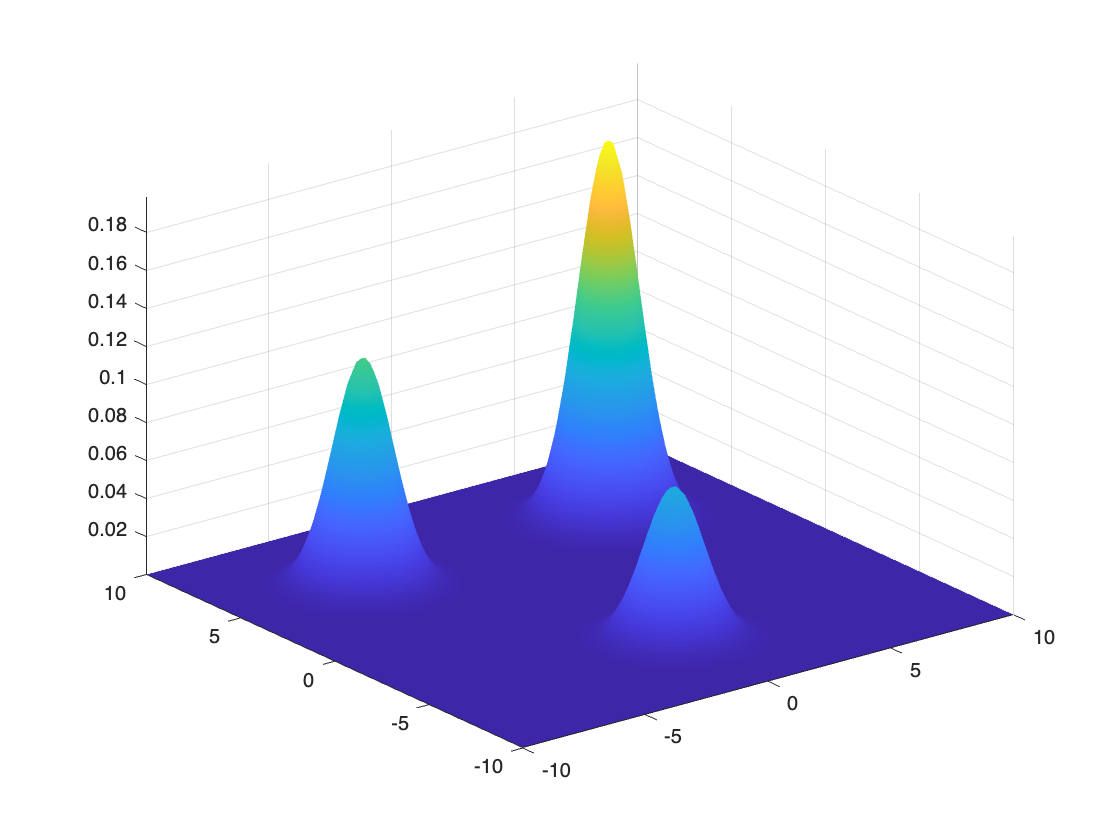
\includegraphics[width=.6\linewidth]{figures/gaussian-mixture.png}
  \caption{An example of a Gaussian mixture with three components. The first component is centered at $[0, -5]^\intercal$ with weight $0.2$, the second component has mean in $[-5, 5]^\intercal$ with weight $0.3$ and the last has mean $[5, 5]^\intercal$ and the weight $0.5$.}
  \label{fig:gaussian-mixture}
\end{figure}

Since the weights sum to one, the Gaussian mixture satisfies the normalization requirement of pdfs and is thus a valid probability density function itself. The weights in the mixture represent the relative importance of the corresponding component. Gaussian mixtures are used to model complex distributions and have several nice mathematical properties as the Gaussian distribution, as we will later see. That is why Gaussian mixtures are widely used to represent posterior distributions in many MTT filters. Moreover, one can easily approximate any distribution with a Gaussian mixture using algorithms such as the Expectation-Maximization algorithm.

A mixture $f(\mathbf{X})$ with $N$ components will have the expected value $\boldsymbol{\hat{\mu}}$ and the covariance $\hat{\Sigma}$ according to the following equations:

\begin{align}
    \boldsymbol{\hat{\mu}} &= \sum_{i=1}^N w_i \boldsymbol{\mu}_i, \\
    \hat{\Sigma} &= \sum_{i=1}^N w_i \Sigma_i + \Tilde{\Sigma},
\end{align}

\noindent where the term $\Tilde{\Sigma}$ is called the spread-of-the-innovations and is defined as:

\begin{equation}
    \Tilde{\Sigma}= \sum_{i=1}^N
        w_i (\boldsymbol{\mu}_i - \hat{\boldsymbol{\mu}})
        (\boldsymbol{\mu}_i - \hat{\boldsymbol{\mu}})^\intercal.
\end{equation}

The spread-of-the-innovations quantifies the magnitude of the difference between expectations of individual components.

        \subsection{State-space model}\label{sec:state-space}
            In the previous section, we established the relationships between prior and 
posterior distributions and learned about recursive Bayesian estimation of the 
posterior. Now, we will explore these concepts in the context of object 
tracking.

Object tracking involves estimating the internal states of objects that move in 
some space, which are often unknown to us. These states may include physical 
properties of objects such as position, velocity, acceleration, and 
orientation, depending on the application. Sensors such as cameras, infrared 
scanners, lidars or radars constantly generate measurements of the object 
states, which may be the distance of an object to the sensor, or its 
temperature. However, these measurements are often noisy due to environmental 
conditions or imperfections of the sensor. We use Bayesian filtering to 
estimate the real state of the objects and filter out the noise.

To handle the complexity and diversity of possible situations and properties, 
we need a systematic framework for modeling object motion that captures all 
sources of uncertainty and the nature of physical behavior of objects. This 
framework is called state-space modeling. In state-space models, the internal 
state we want to estimate is represented as a vector of variables that evolve 
over time according to a set of rules specified by the \textit{motion model}, 
which is a known function. The measurements obtained at each time step are 
modeled as a different function of the state variables, known as the 
\textit{measurement model}\footnote{
    It should be mentioned that the names `motion' and `measurement' models are 
    not the only terms used to describe them. The reader may also encounter 
    terms such as kinematic, state-transition, dynamic, or system models for the 
    motion model, and terms like observation, sensor, or likelihood models for 
    the measurement model. All of these names are correct, and their use depends 
    on the context in which they are applied. However, in this work, the author 
    strives for consistency and will use the terms `motion' and `measurement' 
    models throughout the entire text.
}.

For example, consider a moving bicycle and a surveillance camera with a 
rectangular field of view (FoV). The bicycle enters the FoV and crosses it at a 
constant speed. The camera has an algorithm that estimates the position of 
objects in the space from the image. With each frame $f$, it returns a new 
position, say $(\hat x_f, \hat y_f)$. We can represent the state of the bicycle 
as a vector of the position and velocity, which are unknown variables. Based on 
the measurements, we estimate their values using the known physical relation 
between distance, velocity, and time: $d = v \Delta t$, where $d$ is the 
distance that the object with velocity $v$ traveled in time $\Delta t$.

Both the motion and measurement models should include some noise. In the 
example above, the movement of the bicycle cannot perfectly follow the formula, 
and there will always be some minor changes in speed. Moreover, the measurement 
model, which translates an estimated state into a measurement, will also 
contain some uncertainty since the camera does not have a perfect 
representation of the space.

We can now describe these models formally. Note that since the state is a 
vector, we will use $\mathbf{x}$ for vectors. The motion and measurement models 
can be generally expressed as:

\begin{align}
    p(\vecat{x}{k} | \vecat{x}{k-1}) 
        &= f_t(\vecat{x}{k-1}, \vecat{u}{k}, \vecat{w}{k}), \\
    p(\vecat{z}{k} | \vecat{x}{k}) 
        &= h_t(\vecat{x}{k}, \vecat{v}{k}),
\end{align}

\noindent where $f_t$ and $h_t$ are functions, $\vecat{x}{k-1}$ is the estimated state 
from time step $k-1$, $\vecat{u}{k}$ is called the input (or control) vector, 
and $\vecat{w}{k}$ and $\vecat{v}{k}$ are zero-mean noise random variables.

However, this definition is too general since the functions $f_t$ and $h_t$ can 
be anything. As mentioned earlier, to get a closed-form solution in the 
Bayesian inference framework, we need to choose conjugate distributions for the 
likelihood and the prior. The Kalman filter, which we will describe soon, works 
for the Gaussian-linear case, where the functions $f_t$ and $h_t$ are linear 
and noise variables are distributed as Gaussian, i.e., 
$\vecat{w}{k}, \vecat{v}{k} \sim \mathscr{N}(\mathbf{0}, \Sigma)$. The Gaussian-
linear state-space model has the following representation:

\begin{align}
    p(\vecat{x}{k} | \vecat{x}{k-1}) 
        &= \mathbf{F} \vecat{x}{k-1}
            + \mathbf{B} \vecat{u}{k}
            + \vecat{w}{k},
        & \vecat{v}{k} \sim \mathscr{N}(\mathbf{0}, \mathbf{Q}), \\
    p(\vecat{z}{k} | \vecat{x}{k})
        &= \mathbf{H} \vecat{x}{k} + \vecat{v}{k},
        & \vecat{w}{k} \sim \mathscr{N}(\mathbf{0}, \mathbf{R}), \\
    p(\vecat{x}{0}) &\sim \mathscr{N}(\vecat{\hat{x}}{0}), \vecat{P}{0}),&
\end{align}

\noindent where:

\begin{itemize}
    \item $\mathbf{F}$ is the \textit{transition matrix},
    \item $\mathbf{B}$ is the \textit{input matrix},
    \item $\mathbf{H}$ is the \textit{measurement matrix},
    \item $\mathbf{Q}$ and $\mathbf{R}$ are symmetric positive definite matrices
        that describe the statistical properties of the motion noise
        \vecat{v}{k} and the measurement noise \vecat{w}{k}, respectively,
    \item $\vecat{\hat x}{0}$ and $\vecat{P}{0}$ are mean and variance of the 
    prior state.
\end{itemize}

The control variable $\vecat{u}{k}$, in general, represents some input signal from the environment, and $\mathbf{B}$ specifies how the input signal affects the dynamic system. This may include the effect of gravity on the vertical traveled distance or the voltage applied to some circuit. However, in object tracking, we rely on measurements obtained from sensors to update our estimate of the object's state. We do not have control over the object's motion. Thus, the input matrix is often redundant, and we omit it (or set it to a zero matrix) along with the input variable $\vecat{u}{k}$.

The notation above may be inconvenient in some cases. In this work, we will often use a shorter version that has the same meaning:

\begin{align}
    p(\vecat{x}{k} | \vecat{x}{k-1})
        &= \mathscr{N}(\vecat{x}{k}; \mathbf{F}\vecat{x}{k-1}, \mathbf{Q}), 
        \label{eq:motion-model} \\
    p(\vecat{z}{k} | \vecat{x}{k})
        &= \mathscr{N}(\vecat{z}{k}; \mathbf{H}\vecat{x}{k}, \mathbf{R}), 
        \label{eq:measurement-model} \\
    \vecat{x}{0}
        &\sim \mathscr{N}(\vecat{x}{0}; \vecat{\hat{x}}{0}, \vecat{P}{0}).
        \label{eq:prior-x0}
\end{align}

            \subsubsection{Constant Velocity Model}\label{sec:cv-model}
                The Constant Velocity (CV) model is one of the most commonly used motion and measurement models in the context of object tracking. It describes the kinematics of objects in a 2D space that move with a constant velocity. The state vector comprises a position vector and a velocity vector, and while the position vector contains the coordinates of the object in the space, the velocity vector contains the object speed in the direction of each axis.

The CV model is linear and one of the simplest models. It assumes that the speed of objects remains unchanged during tracking, with only small deviations from the constant. This model can be reasonably utilized in scenarios where objects do not change their speed or direction, such as vehicles on highways or planes in the sky. Since the state vector contains only four variables, the use of this model does not increase the computational burden on tracking algorithms.

The motion equation for the CV model is given by \ref{eq:motion-model}, and the state vector $\vecat{x}{k}$, the state transition matrix $\mathbf{F}$, and the process noise matrix $\mathbf{Q}$ can be defined as:

\begin{equation}
    \vecat{x}{k} =
    \begin{bmatrix}
        x_{1,k} \\ 
        x_{2,k} \\ 
        v_{x_1,k} \\ 
        v_{x_2,k}
    \end{bmatrix};
    \quad
    \mathbf{F} =
    \begin{bmatrix}
       1 & 0 & dt & 0 \\
       0 & 1 & 0 & dt \\
       0 & 0 & 1 &  0 \\
       0 & 0 & 0 &  1 
    \end{bmatrix};
    \quad
    \mathbf{Q} = q^2 \cdot
    \begin{bmatrix}
        \frac{dt^3}{3}    & 0                 & \frac{dt^{2}}{2}  & 0  \\
        0                 & \frac{dt^3}{3}    & 0                 & \frac{dt^{2}}{2} \\
        \frac{dt^{2}}{2}  & 0                 & dt                & 0 \\
        0                 & \frac{dt^{2}}{2}  & 0                 & dt
    \end{bmatrix},
\end{equation}

\noindent where $dt$ is the change in time between the last estimation and the newly computed one, and $q$ is the motion noise parameter, which represents the uncertainty in the state transition.

The measurement model transforms a state vector from the state space into the measurement space. Since the vanilla Kalman filter, which we will derive soon, works only with linear models, the measurement model for the CV model assumes sensors measurements in the same 2D space as in the state vectors. The measurement equation is given by \ref{eq:measurement-model}, and the measurement matrix $\mathbf{H}$ and the measurement noise matrix $\mathbf{R}$ can be defined as:

\begin{equation}
    H =
    \begin{bmatrix}
        1 & 0 &0 & 0 \\
        0 & 1 &0 & 0
    \end{bmatrix};
    \quad
    R =
    r^{2}\cdot
    \begin{bmatrix}
        1 & 0 \\
        0 & 1
    \end{bmatrix},
\end{equation}

\noindent where $r$ is the measurement noise parameter, which determines the variance of the measurement noise.

We need to describe the choice of parameters $q$ and $r$ in more detail. These parameters are crucial in obtaining good estimates from a filter. These parameters are not known a priori and their values should be chosen carefully by the means of trial and error, or using automated methods like, for instance, in \cite{bulutProcessMeasurementNoise2011}. However, selecting appropriate values often involves a trade-off between tracking accuracy and computational complexity, and the use of exact methods depends on the application and one's requirements.

The CV model can be extended with additional information, such as change of speed. In this way we will come to the constant acceleration model. However, it will not be used in this work and, therefore, we will not leave formal definition of this model here.

        \subsection{The Bayes filter}\label{sec:bayes-filter}
            We have learned how the internal state of a system can be represented in terms
of a state vector and motion and measurement models. Now, we are ready to 
present the formal definition of the Bayes filter, the general abstraction of
any Bayesian filter, including the Kalman filter and the PHD filter.

First, we need to make a very important assumption on states. This assumption
is called the \textit{Markov model property}. This property states that, for 
the motion model, the present state of a system $x_k$ is dependent only on 
the state on the previous time step $x_{k-1}$ given all past states $x_{1:k-1}$ 
and measurements $z_{1:k-1}$. More formally:

\begin{equation}
p(x_k | x_1, \ldots, x_{k-2}, x_{k-1},
        z_1, \ldots, z_{k-2}, z_{k-1}) 
    = p(x_k | x_{k-1}).
\end{equation}

A similar requirement must hold for measurement model, that is:

\begin{equation}
    p(z_k | x_1, \ldots, x_{k-2}, x_{k-1}, x_{k}
        z_1, \ldots, z_{k-2}, z_{k-1}) 
    = p(z_k | x_k).
\end{equation}

The Markov property may seem restrictive but in reality it is not because state-
space models allows us to capture dependencies in the system dynamics by simply 
introducing more variables into the state vector. For instance, if we have a 
system where the current state has a dependence on the previous two states, we 
can augment the state vector to include the last two states as variables, and 
the Markov property will still hold.

The Bayes filter uses the motion and measurement models and assumes that this
property holds. The Bayes filter is a recursive framework that estimates an
internal state of the system over time using measurements. Every iteration of
the filter consists of two steps: prediction and update. On the prediction step,
the filter estimates a internal state $x_k$ based on the previous state
$x_{k-1}$ and the motion model $p(x_k | x_{k-1})$. The prediction step
is also known as the Chapman-Kolmogorov equation.

\begin{theorem}[The prediction step. The Chapman-Kolmogorov equation]\label{theorem:bayes-filter-predict}\label{theorem:chapman-kolmogorov}
    Given the set of measurements $z_{1:k-1} = \{z_1, z_2, \ldots, z_{k-1}\}$ 
    and the current state $x_{k-1}$ and the motion model $p(x_k | x_{k-1})$, 
    the prediction step of the Bayes filter is computed as follows:

    \begin{equation}
        p\left({x}_k | {z}_{1: k-1}\right)
        = \int 
            p\left(
                {x}_k, {x}_{k-1} | {z}_{1: k-1}
            \right)
            \mathrm{d} {x}_{k-1}
        = \int
            p\left(
                {x}_k | {x}_{k-1}\right
            ) p\left(
                {x}_{k-1} | {z}_{1: k-1}
            \right)
            \mathrm{d} {x}_{k-1}.
    \end{equation}
\end{theorem}

Next, on the update step, the filter corrects the predicted state with the 
measurement $z_k$ using the measurement model $p(z_k | x_k)$. This step is
computed using the standard Bayes' rule.

\begin{theorem}[The update step]\label{theorem:bayes-filter-update}
    Given the output of the prediction step of the Bayes filter 
    $p\left({x}_k | {z}_{1: k-1}\right)$, the observed measurement $z_k$
    and the measurement model $p(z_k | x_k)$, the update step of the Bayes
    filter is computed as follows:
    
    \begin{equation}
        p\left({x}_k | {z}_{1: k}\right)=\frac{p\left({z}_k | {x}_k\right) p\left({x}_k | {z}_{1: k-1}\right)}{p\left({z}_k | {z}_{1: k-1}\right)} \propto p\left({z}_k | {x}_k\right) p\left({x}_k | {z}_{1: k-1}\right).
    \end{equation}
\end{theorem}

These two steps create a loop, and to use the filter, we first predict the next state using the Chapman-Kolmogorov equation, and then we update our guess with a measurement. Note, that we will often use the simplified notation to explicitly state the time step of the value. The notation $\vecat{\bullet}{k|k-1}$ represents the predicted value at time step $k$, and the notation $\vecat{\bullet}{k|k}$ represents the updated value at time step $k$ after incorporating a measurement.

Now, having introduced the general Bayes filter, we will continue with 
exploring the Kalman filter in detail, the popular and widely used tool for 
state estimation.

        \subsection{The Kalman filter}\label{sec:kf-index}
            The Kalman filter is one of the most well-known and widely used algorithms in 
signal processing and control theory. It is a recursive algorithm that allows 
the estimation of internal states of entities in dynamic systems from a set of 
measurements that may be noisy or missing at some time steps. The filter was 
proposed by Rudolf Kalman in 1960 \cite{kalmanNewApproachLinear1960} and has 
since been pervasively used to control a vast array of consumer, health, 
commercial, and defense products \cite{grewalApplicationsKalmanFiltering2010}.

The development of the filter was motivated by the need to improve aerospace 
technology in the United States during the Cold War between the Soviet Block 
and the North American Treaty Organization. Because the Soviet Union managed to 
launch its artificial satellites and successfully send a human to space, the 
federal government of the United States supported research into new 
technologies in the aerospace area.

The Kalman filter is an example of a general Bayes filter that was introduced 
earlier. This means that the filter estimates the posterior distribution of the 
internal state at discrete time steps using prior information about the 
observed object's state and a set of noisy measurements. As briefly mentioned 
in Section \ref{sec:state-space}, the Kalman filter works on state-space linear 
models with Gaussian noise and a Gaussian prior of the state. The predict-
update loop in the Kalman filter is the same as in the Bayes filter, and the 
same Chapman-Kolmogorov equation defined in \ref{theorem:chapman-kolmogorov} 
and the update equation defined in \ref{theorem:bayes-filter-update} are 
incorporated.

The main advantage of the Kalman filter is that it allows for the estimation of 
the state of a system in real-time. It handles noisy measurements well and is 
fast; however, it is sensitive to initial parameter settings, such as the noise 
covariance matrices \cite{gePerformanceAnalysisKalman2016}. Nonetheless, there 
are new methods being developed that propose mechanisms to overcome this 
drawback, as in \cite{matiskoNoiseCovariancesEstimation2010} and 
\cite{yuenOnlineEstimationNoise2013}.

One of the main drawbacks of the Kalman filter is its Gaussian-linear 
assumption. In real-world applications, many systems exhibit non-linearity, and 
the Kalman filter may be ineffective. Nonetheless, several extensions of the 
filter have been proposed that address this. Two well-known algorithms are the 
Unscented Kalman Filter (UKF) and the Extended Kalman filter (EKF). The UKF is 
an algorithm that uses a set of carefully chosen sigma points to capture the 
true mean and covariance of the predicted and updated distributions without 
the need for linearization \cite{wanUnscentedKalmanFilter2000}. The EKF, on 
the other hand, linearizes the nonlinear motion and measurement models using a 
first-order Taylor expansion \cite{smithApplicationStatisticalFilter1962}. 
These methods have been proven to be effective in many applications, including 
the PHD filter. However, they are beyond the scope of this thesis and will not 
be covered in detail.

            \subsubsection{The Gaussian identity}\label{sec:gaussian-identity}
                Before we introduce the actual formulas of the Kalman filter, we should introduce a new fundamental theorem in object tracking and then deduce a corollary from it. These will also be used later when we infer formulas for the the GM-PHD filter. We define this theorem using a general notation without any meaning for Bayesian filters to avoid the confusion of variables when we use this theorem in different parts of different filters.

\begin{theorem}[The Gaussian product identity]\label{theorem:gaussian-identity}
    Given matrices and vectors $A, U, m, d$, and $V$ of appropriate dimensions, and that $U$ and $V$ are positive definite, the following identity applies:

    \begin{equation}\label{eq:gid}
        \mathscr{N}(x ; A y + d, U) \mathscr{N}(y ; m, V)=\mathscr{N}(x ; A m + d, U + A V A^\intercal) \mathscr{N}(y ; \hat{m}, \hat{V}),
    \end{equation}

    \noindent where
    \begin{align}
        \hat{m} & = m + K (y - Am - d), \\ 
        \hat{V} & = (I - K A) V, \\
        K &= V A^\intercal (U + A V A^\intercal)^{-1}.
    \end{align}
\end{theorem}

\begin{proof}\label{proof:gaussian-identity}
    The proof of Theorem \ref{theorem:gaussian-identity} presented here follows similar proofs in \cite{mahlerStatisticalMultisourcemultitargetInformation2007} (Appendix D) and \cite{risticKalmanFilterParticle2004} (Section 3.8). However, the main idea of using algebraic manipulation of matrices was taken from \cite{tokleMultiTargetTracking2018}.
    
    The proof is based on the idea that both sides of \ref{eq:gid} represent the joint Gaussian distribution of two random variables, $p(x,y)$. From \ref{def:cond-prob-pdf}, we know that we can express this distribution as:
    
    \begin{equation}
        p(x, y) = p(x|y)p(y) = p(y|x)p(x).
    \end{equation}
    
    We claim that the left-hand side (LHS) of \ref{eq:gid} represents this equality, i.e.,
    
    \begin{equation}
        p(x, y) = p(x|y)p(y) = \mathscr{N}(x ; A y + d, U) \mathscr{N}(y ; m, V).
    \end{equation}

    Next, we can express the product of two Gaussians in their quadratic forms, the same form as defined in \ref{eq:vec-gauss-def}, i.e.

    \begin{align}
        \mathscr{N}(x ; A y + d, U) \mathscr{N}(y ; m, V)
        &= \frac{1}{(2\pi)^{n} \sqrt{|U| |V|}}
        \exp \left(
        -\frac{1}{2}
        \bigg[(x - Ay - d)^\intercal U^{-1} (x - Ay - d) \right. \nonumber \\
        &\left.\qquad\qquad\qquad\qquad\qquad+ (y - m)^\intercal V^{-1} (y - m) \bigg] \right).
        \label{eq:gid-proof:lhs-expanded}
    \end{align}

    If we introduce a small algebraic trick for matrices:

    \begin{equation}
        \begin{bmatrix}
            I & -A \\
            0 & I
        \end{bmatrix}
        \begin{bmatrix}
            x - Am - d \\
            y - m
        \end{bmatrix}
        =
        \begin{bmatrix}
            x - Am - d - Ay + Am \\
            y - m \\
        \end{bmatrix}
        =
        \begin{bmatrix}
            x - Ay - d \\
            y - m
        \end{bmatrix},
    \end{equation}
    
    we can manipulate the exponent to obtain another quadratic form:

    \begin{align}
        &\phantom{=}
        (x - Ay - d)^\intercal U^{-1} (x - Ay - d) + (y - m)^\intercal V^{-1} (y - m) 
        \nonumber \\
        &=
        \begin{bmatrix}
            x - Ay - d \\
            y - m
        \end{bmatrix}^\intercal
        \begin{bmatrix}
            U^{-1} & 0 \\
            0 & V^{-1}
        \end{bmatrix}
        \begin{bmatrix}
            x - Ay - d \\
            y - m
        \end{bmatrix}
        \nonumber \\
        &=
        \begin{bmatrix}
            x - Am - d \\
            y - m
        \end{bmatrix}^\intercal
        \begin{bmatrix}
            I & 0 \\
            -A^\intercal & I
        \end{bmatrix}
        \begin{bmatrix}
            U^{-1} & 0 \\
            0 & V^{-1}
        \end{bmatrix}
        \begin{bmatrix}
            I & -A \\
            0 & I
        \end{bmatrix}
        \begin{bmatrix}
            x - Am - d \\
            y - m
        \end{bmatrix}
        \nonumber \\
        &=
        \begin{bmatrix}
            x - Am - d \\
            y - m
        \end{bmatrix}^\intercal
        \left(
        \begin{bmatrix}
            I & A \\
            0 & I
        \end{bmatrix}
        \begin{bmatrix}
            U & 0 \\
            0 & V
        \end{bmatrix}
        \begin{bmatrix}
            I & 0 \\
            A^\intercal & I
        \end{bmatrix}
        \right)^{-1}
        \begin{bmatrix}
            x - Am - d \\
            y - m
        \end{bmatrix}
        \nonumber \\
        &=
        \begin{bmatrix}
            x - Am - d \\
            y - m
        \end{bmatrix}^\intercal
        \begin{bmatrix}
            U + A V A^\intercal & A V \\
            V A^\intercal & V
        \end{bmatrix}^{-1}
        \begin{bmatrix}
            x - Am - d \\
            y - m
        \end{bmatrix}. \label{eq:gid-proof-quadratic-form}
    \end{align}

    This expression is also a joint Gaussian distribution $p(x,y)$, but it cannot be split into two independent Gaussians due to the fact that the matrix is not block-diagonal. Therefore, to conclude the proof, we need to infer two other distributions, $p(y|x)$ and $p(x)$, from the derived distribution $p(x, y)$.
    
    Notice that this is also a quadratic form, and it expresses a dependency on both $x$ and $y$. Therefore, his expression is also a joint Gaussian distribution $p(x,y)$, but it cannot be split into two independent Gaussians due to the fact that the covariance matrix in \ref{eq:gid-proof-quadratic-form} is not block-diagonal. Therefore, to conclude the proof, we need to infer two other distributions, $p(y|x)$ and $p(x)$, from the derived distribution $p(x, y)$.
    
    We are going to obtain the $p(y|x)$ distribution by conditioning on the joint distribution, i.e. using the formula that was presented in Theorem \ref{theorem:gauss-marg}. For completeness and simplicity, we will write the joint distribution the same way that it is presented in the theorem:

    \begin{equation}
        p(x,y) = 
        \mathscr{N}\left(
            \begin{bmatrix}
                x \\
                y
            \end{bmatrix}
            ;
            \begin{bmatrix}
                Am + d \\
                m
            \end{bmatrix}
            ,
            \begin{bmatrix}
                U + A V A^\intercal & A V \\
                V A^\intercal & V
            \end{bmatrix}
        \right).
    \end{equation}

    Now, using equations \ref{eq:gauss-cond} and \ref{eq:gauss-cond-params}, we will infer:

    \begin{align}
        \mu_{y|x}
        &= \mu_y + \Sigma_{yx} \Sigma_{xx}^{-1}(x - \mu_x) \nonumber \\
        &= m + V A^\intercal (U + A V A^\intercal)^{-1}(x - Am - d), \\
        \Sigma_{y|x}
        &= \Sigma_{yy} - \Sigma{yx}\Sigma_{xx}^{-1}\Sigma_{yx} \nonumber \\
        &= V - V A^\intercal (U + A V A^\intercal)^{-1} A V \nonumber \\
        &= (I - V A^\intercal (U + A V A^\intercal)^{-1} A) V, \\
        p(y|x)
        &= \mathscr{N}\left(y; \mu_{y|x}, \Sigma_{y|x}\right).
    \end{align}

    Using Theorem \ref{theorem:gauss-marg}, we obtain the expression for $p(x)$:

    \begin{equation}
        p(x) = \mathscr{N}(x; Am + d, U + A V A^\intercal).
    \end{equation}

    If we introduce a new notation, $K = V A^\intercal (U + A V A^\intercal)^{-1}$, we obtain the exact same expressions for the Gaussians on the right-hand side (RHS) of the initial theorem. That confirms that both LHS and RHS are equal due to the equivalence of their quadratic forms. And that concludes the proof.
\end{proof}

From Theorem \ref{theorem:gaussian-identity} we can also derive a corollary, that we will also need.

\begin{corollary}\label{theorem:gid-integral}
    Given matrices and vectors $A, U, m, d$, and $V$ of appropriate dimensions, and that $U$ and $V$ are positive definite, the following identity applies:

    \begin{equation}\label{eq:gid-integral}
        \int \mathscr{N}(x ; A y + d, U) \mathscr{N}(y ; m, V) \mathrm{d}y=\mathscr{N}(x ; A m + d, U + A V A^\intercal).
    \end{equation}
\end{corollary}

\begin{proof}
    The proof of Corollary \ref{theorem:gid-integral} is straightforward:

    \begin{align}
        \int \mathscr{N}(x ; A y + d, U) \mathscr{N}(y ; m, V) \mathrm{d}y 
        &= \int \mathscr{N}(x ; A m + d, U + A V A^\intercal) \mathscr{N}(y ; \hat{m}, \hat{V}) \mathrm{d}y \label{eq:git-int-proof-step1} \\
        &= \mathscr{N}(x ; A m + d, U + A V A^\intercal) \underbrace{\int \mathscr{N}(y ; \hat{m}, \hat{V}) \mathrm{d}y}_{\text{=1}} \label{eq:git-int-proof-step2}\\
        &= \mathscr{N}(x ; A m + d, U + A V A^\intercal). \label{eq:git-int-proof-step3}
    \end{align}

    In \ref{eq:git-int-proof-step1}, we applied Equation \ref{eq:gid} from Theorem \ref{theorem:gaussian-identity}, then, in \ref{eq:git-int-proof-step2} we notice that one of the integrands does not depend on the integration variable $y$ and we take it out from the integral. The integrand that is left under the integral is a Gaussian distribution probability density function, and it integrates to $1$. Equation \ref{eq:git-int-proof-step3} is the right-hand side of Equation \ref{eq:gid-integral}. It concludes the proof of Corollary \ref{theorem:gid-integral}.
\end{proof}

            \subsubsection{The Kalman filter algorithm}\label{sec:kf-algorithm}
                We have derived several important formulas and relations, which are essential to infer the formulas and algorithm of the Kalman filter. We should recall that the filter has Gaussian-linear motion and measurement models and is essentially a Bayesian filter. The formal description of the linear models was given in \ref{eq:motion-model} and \ref{eq:measurement-model}, the prediction step of the Bayesian filter in Theorem \ref{theorem:bayes-filter-predict}, and the update step in Theorem \ref{theorem:bayes-filter-update}. With all the necessary pieces in place, we can now derive the prediction and update formulas for the Kalman filter.

\begin{theorem}[The Kalman filter prediction]\label{theorem:kalman-predict}
    Assume that the motion and measurement models are given by \ref{eq:motion-model} and \ref{eq:measurement-model}, respectively, and that the Markov assumption of the Bayes filter holds, so that the Chapman-Kolmogorov equation is applicable. Let the posterior density at time step $k-1$ be denoted as $\mathscr{N}(\vecat{x}{k-1}; \vecat{\hat{x}}{k-1|k-1}, \vecat{P}{k-1|k-1})$. Then, the predicted density is given by:

    \begin{equation}
        p\left(\vecat{x}{k} | \vecat{z}{1:k-1}\right)
        = \mathscr{N}\left(
                \vecat{x}{k};
                \mathbf{F} \vecat{\hat{x}}{k-1|k-1},
                \mathbf{F} \vecat{P}{k-1|k-1} \mathbf{F}^\intercal + \mathbf{Q}
            \right).
    \end{equation}
\end{theorem}

\begin{proof}
    \begin{align}
        p\left(\vecat{x}{k} | \vecat{z}{1:k-1}\right)
        &= \int
            p\left(
                \vecat{x}{k} | \vecat{x}{k-1}\right)
            p\left(
                \vecat{x}{k-1} | \vecat{z}{1:k-1}
            \right)
            \mathrm{d} \vecat{x}{k-1} \label{eq:kf-pred-s1} \\
        &= \int
            \mathscr{N}\left(
                \vecat{x}{k}; \mathbf{F}\vecat{x}{k-1}, \mathbf{Q}
            \right)
            \mathscr{N}\left(
                \vecat{x}{k-1}; \vecat{\hat{x}}{k-1|k-1}, \vecat{P}{k-1|k-1}
            \right)
            \mathrm{d} \vecat{x}{k-1} \label{eq:kf-pred-s2} \\
        &= \int
            \mathscr{N}\left(
                \vecat{x}{k};
                \mathbf{F} \vecat{\hat{x}}{k-1|k-1},
                \mathbf{Q} + \mathbf{F} \vecat{P}{k-1|k-1} \mathbf{F}^\intercal
            \right)
            \mathscr{N}\left(
                \vecat{x}{k-1}; \bullet, \bullet
            \right)
            \mathrm{d} \vecat{x}{k-1} \label{eq:kf-predict-gauss-id}\\
        &= \mathscr{N}\left(
                \vecat{x}{k};
                \mathbf{F} \vecat{\hat{x}}{k-1},
                \mathbf{F} \vecat{P}{k-1} \mathbf{F}^\intercal + \mathbf{Q}
            \right). \label{eq:kf-predict-result}
    \end{align}

    We started with the application of the Chapman-Kolmogorov equation from \ref{theorem:chapman-kolmogorov} and the substitution of its terms with the suitable distributions. Next, in the equation \ref{eq:kf-predict-result}, we used the result of Theorem \ref{theorem:gaussian-identity}, and finally we applied Corollary \ref{theorem:gid-integral} to get \ref{eq:kf-predict-result}.
\end{proof}

\begin{theorem}[The Kalman filter update]\label{theorem:kalman-update}
    Assume that the predicted density from \ref{theorem:kalman-predict} is $p\left(\vecat{x}{k} | \vecat{z}{1:k-1}\right)=\allowbreak \mathscr{N}\left(\vecat{x}{k}; \mathbf{F} \vecat{\hat{x}}{k|k-1}, \mathbf{F} \vecat{P}{k|k-1} \mathbf{F}^\intercal + \mathbf{Q}\right)$, $p(\vecat{z}{k} | \vecat{x}{k})$ is the measurement model given in \ref{eq:measurement-model},
    and $\vecat{z}{k}$ is the measurement at time $k$. Then the posterior density after the update step is given by the following relation:

    \begin{equation}
        p(\vecat{x}{k} | \vecat{z}{k}) = 
        \mathscr{N}\left(
            \vecat{x}{k}; \vecat{\hat{x}}{k|k}, \vecat{P}{k|k}
        \right),
    \end{equation}

    where the mean and covariance are given by:

    \begin{align}
        \vecat{\hat{x}}{k|k}
        &= \vecat{\hat{x}}{k|k-1} + \vecat{K}{k}(\vecat{z}{k} - \mathbf{H}\vecat{\hat{x}}{k|k-1}), \\
        \vecat{P}{k|k}
        &= (\mathbf{I} - \vecat{K}{k}\mathbf{H})\vecat{P}{k|k-1}, \\
        \vecat{K}{k} 
        &= \vecat{P}{k|k-1}\mathbf{H}^\intercal(\mathbf{H}\vecat{P}{k|k-1}\mathbf{H}^\intercal + \mathbf{R})^{-1}.
    \end{align}
\end{theorem}

\begin{proof}
    \begin{align}
        p(\vecat{x}{k} | \vecat{z}{k})
        &= p(\vecat{z}{k} | \vecat{x}{k}) p(\vecat{x}{k}) \\
        &= p(\vecat{z}{k} | \vecat{x}{k}) p(\vecat{x}{k} | \vecat{z}{1:k-1}) \\
        &= \frac{
            \mathscr{N}\left(\vecat{z}{k}; \mathbf{H} \vecat{x}{k}, R\right)
            \mathscr{N}\left(\vecat{x}{k}; \vecat{\hat{x}}{k|k-1}, \vecat{P}{k|k-1} \right)
        }{
            \int
            \mathscr{N}\left(\vecat{z}{k}; \mathbf{H} \vecat{x}{k}, R\right)
            \mathscr{N}\left(\vecat{x}{k}; \vecat{\hat{x}}{k|k-1}, \vecat{P}{k|k-1} \right)
            \mathrm{d} \vecat{x}{k}
        } \\
        &= \frac{
            \mathscr{N}\left(\vecat{z}{k}; \mathbf{H} \vecat{\hat{x}}{k|k-1}, \mathbf{H} \vecat{P}{k|k-1} \mathbf{H}^\intercal + \mathbf{R}\right)
            \mathscr{N}\left(\vecat{x}{k}; \vecat{\hat{x}}{k|k}, \vecat{P}{k|k} \right)
        }{
            \mathscr{N}\left(\vecat{z}{k}; \mathbf{H} \vecat{\hat{x}}{k|k-1}, \mathbf{H} \vecat{P}{k|k-1} \mathbf{H}^\intercal + \mathbf{R}\right)
        } \\
        &= \mathscr{N}\left(\vecat{x}{k}; \vecat{\hat{x}}{k|k}, \vecat{P}{k|k} \right),
    \end{align}

    where, according to Theorem \ref{theorem:gaussian-identity}, the values of $\vecat{\hat{x}}{k|k}$ and $\vecat{P}{k|k}$ are:

    \begin{align}
        \vecat{\hat{x}}{k|k}
        &= \vecat{\hat{x}}{k|k-1} + \vecat{K}{k}(\vecat{z}{k} - \mathbf{H}\vecat{\hat{x}}{k|k-1}), \\
        \vecat{P}{k|k}
        &= (\mathbf{I} - \vecat{K}{k}\mathbf{H})\vecat{P}{k|k-1}, \\
        \vecat{K}{k} 
        &= \vecat{P}{k|k-1}\mathbf{H}^\intercal(\mathbf{H}\vecat{P}{k|k-1}\mathbf{H}^\intercal + \mathbf{R})^{-1}.
    \end{align}

    This proof utilizes the same Gaussian product identity theorem with its corollary utilizing in addition the application of the Bayes' rule.
\end{proof}

Before we conclude this section with the full algorithm of the Kalman filter, it should be noted that straightforward computation of the covariance matrix after the update step is sensitive to round-off numerical errors, and this can be avoided using a different form of the same expression for $\vecat{P}{k|k}$ \cite{bar-shalomEstimationApplicationsTracking2001}:

\begin{equation}\label{eq:kf-joseph-form}
    \vecat{P}{k|k} =
    (\mathbf{I} - \vecat{K}{k}\mathbf{H})\vecat{P}{k|k-1}
    (\mathbf{I} - \vecat{K}{k}\mathbf{H})^\intercal
    + \vecat{K}{k} \mathbf{R} \vecat{K}{k}^\intercal.
\end{equation}

This form is called the \textit{Joseph form} and is less sensitive to numerical errors. In the algorithm, we will use this form to compute the covariance matrix after the update step. The whole algorithm of the Kalman filter is defined as follows:

\begin{algorithm}
\caption{Kalman filter algorithm}\label{alg:kf}
\begin{algorithmic}[1]
    \Procedure{KF}{$\vecat{\hat{x}}{k-1|k-1}$, $\vecat{P}{k-1|k-1}$, $\vecat{z}{k}$}
        \State $\vecat{\hat{x}}{k|k-1}, \vecat{P}{k|k-1} 
            \gets \Call{KFPredict}{\vecat{\hat{x}}{k-1|k-1}, \vecat{P}{k-1|k-1}}$
        \State $\vecat{\hat{x}}{k|k}, \vecat{P}{k|k} 
            \gets \Call{KFUpdate}{\vecat{\hat{x}}{k|k-1}, \vecat{P}{k|k-1}}$
        \State \Return $\vecat{\hat{x}}{k|k-1}, \vecat{P}{k|k-1}, \vecat{\hat{x}}{k|k}, \vecat{P}{k|k}$
    \EndProcedure
    
    \item[]
    \Procedure{KFPredict}{$\vecat{\hat{x}}{k-1|k-1}$, $\vecat{P}{k-1|k-1}$}
        \State 
            $\vecat{\hat{x}}{k|k-1} \gets \mathbf{F} \vecat{\hat{x}}{k-1|k-1}$
            \Comment{Predicted state estimate}
        \State
            $\vecat{P}{k|k-1} \gets \mathbf{F} \vecat{P}{k-1|k-1} \mathbf{F}^\intercal + \mathbf{Q}$
            \Comment{Predicted covariance}
        \State \Return $\vecat{\hat{x}}{k|k-1}, \vecat{P}{k|k-1}$
    \EndProcedure

    \item[]
    \Procedure{KFUpdate}{$\vecat{\hat{x}}{k|k-1}$, $\vecat{P}{k|k-1}$}
        \State
            $\vecat{K}{k} \gets \vecat{P}{k|k-1}\mathbf{H}^\intercal(\mathbf{H}\vecat{P}{k|k-1}\mathbf{H}^\intercal + \mathbf{R})^{-1}$
            \Comment{The Kalman gain}
        \State
            $\vecat{\hat{x}}{k|k} \gets \vecat{\hat{x}}{k|k-1} + \vecat{K}{k}(\vecat{z}{k} - \mathbf{H}\vecat{\hat{x}}{k|k-1})$
            \Comment{Posterior state estimate}
        \State
            $\vecat{P}{k|k} \gets (\mathbf{I} - \vecat{K}{k}\mathbf{H})\vecat{P}{k|k-1} (\mathbf{I} - \vecat{K}{k}\mathbf{H})^\intercal + \vecat{K}{k} \mathbf{R} \vecat{K}{k}^\intercal$
            \Comment{Posterior covariance in Joseph form}
        \State \Return $\vecat{\hat{x}}{k|k}, \vecat{P}{k|k}$
    \EndProcedure
\end{algorithmic}
\end{algorithm}

The Kalman filter is the best possible linear estimator in the MMSE (minimum mean square error) sense \cite{humpherysFreshLookKalman2012}. That means that the Kalman filter achieves the minimum expected squared error between the true and estimated values, among all possible linear estimation methods. In other words, assuming the motion model and the measurement model are linear, and the noise is Gaussian and uncorrelated, the filter provides the optimal estimate. However, as it was mentioned before, there are plenty of modifications that allow to use non-linear models or non-Gaussian correlated noise. In this work, we will use the vanilla Kalman filter.


\chapter{Multi-target tracking}\label{ch:mtt}
    % - Multi-object tracking problem, assumptions
%     - Recall some part from Intro, gradually from JPDA to PHD
% - Object birth/survival

In this section, we provide the theoretical background of the multi-target tracking problem. We have already established the foundations of Bayesian filtering and explained in detail how the Kalman filter works. Now, we will discuss how it differs from other filters that are used for tracking objects. Before we start building the theoretical foundations for object tracking filters, we need to clarify the difference between Bayesian filtering and Bayesian object tracking.

When we track objects, we rely on measurements from sensors, such as cameras, lidars, or radars. These sensors have specific technical specifications and limitations, and there is no sensor that can be 100\% reliable. The reliability of a sensor may be affected by noise, which occurs when a sensor detects an object that is not present. This behavior may be caused by weather conditions in the sensor's operating area, the sensor's limited resolution, or dirt or dust covering the sensor's surface. We do not address the exact reasons why this happens; we only need to find ways to eliminate noisy measurements and separate them from measurements generated by existing objects.

The second problem is closely related to the first. It occurs when a sensor fails to generate measurements for objects that are present in its field of view. The reasons for this may be the same as for noisy measurements, and we do not address these reasons directly. However, we must be able to mathematically model these situations to ensure that they can be properly handled by the filter we want to use to track objects.

These two problems have their names that we will use in this work. Noisy measurements are called \textit{clutter}, and missing measurements are called \textit{misdetections}. We have already seen that the latter problem can be handled by the Kalman filter by skipping the update step. Clutter, on the other hand, creates a much more challenging problem. Figure \ref{fig:clutter-intro} shows what clutter looks like to the filter. In the left image, we see a track of an object and measurements generated by the sensor, shown in red. Clutter measurements are shown as blue asterisks. We can distinguish between measurements and clutter. However, in the right image, we see how the filter sees the same data points, with all points in the same color. To the filter, all these points look the same, and there is no easy way to distinguish between clutter and real measurements.

\begin{figure}
\centering
\begin{subfigure}[t]{.45\textwidth}
  \centering
  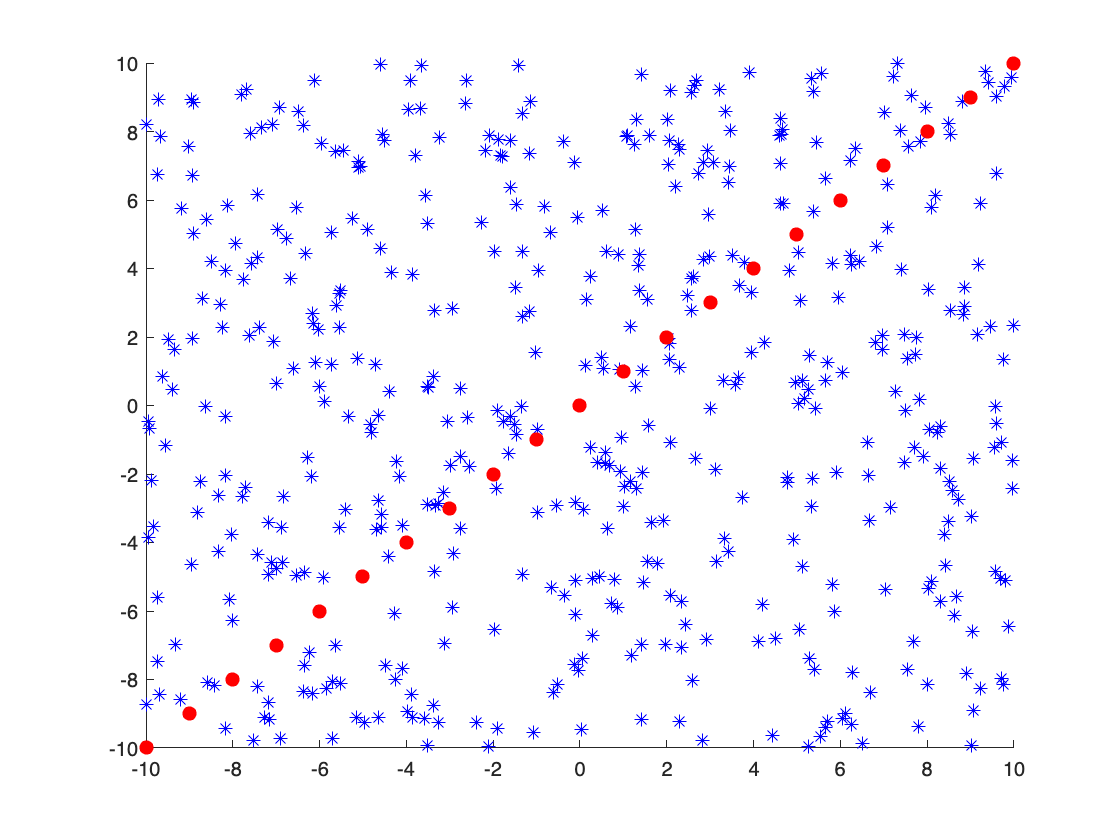
\includegraphics[width=.9\linewidth]{figures/clutter.intro.1.png}
   \caption{Real measurements from some object are shown as red dots. Clutter measurements are displayed as blue asterisks.}
  \label{fig:clutter-intro:1}
\end{subfigure}\hfill
\begin{subfigure}[t]{.45\textwidth}
  \centering
  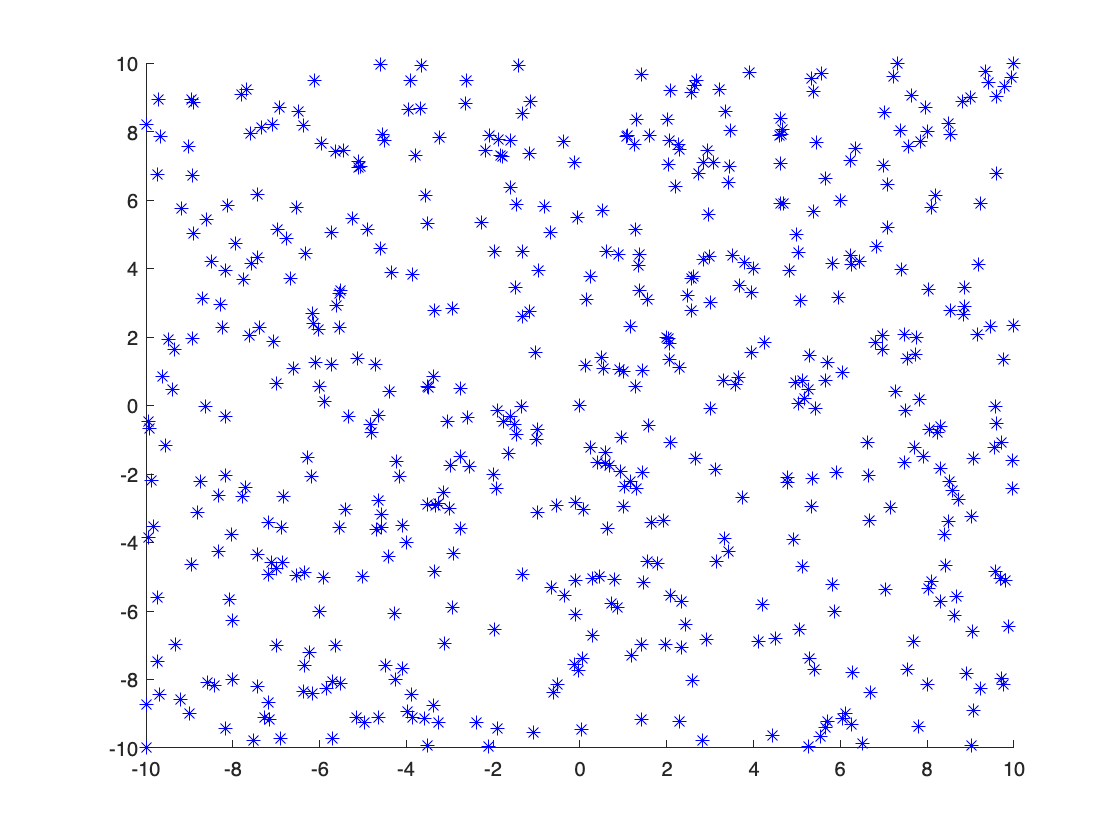
\includegraphics[width=.9\linewidth]{figures/clutter.intro.2.png}
  \caption{Both real measurements and clutter measurements are shown as blue asterisks.}
  \label{fig:clutter-intro:2}
\end{subfigure}
\caption[Measurements in clutter.]{Measurements in clutter. In this Figure, we indicate the clutter problem. When a sensor generates measurements, some of them may be clutter measurements, and there is no easy way to distinguish which data points come from a real object and which are noise.}
\label{fig:clutter-intro}
\end{figure}

The uncertainty in distinguishing between real measurements and clutter has led to the development of many methods for addressing this problem. The main idea behind these methods is that, since we have no information about which measurements come from targets and which are clutter, we should consider all measurements at each time step as coming from a target. This involves creating all possible assignments between measurements and targets and then evaluating the probability of each such assignment. In other words, we evaluate the possibility that a given measurement comes from a specific target according to its motion model. If the measurement is too far from the target, the probability of such an assignment will be lower than that of an assignment with a measurement that is close to the predicted state. These assignments are referred to as \textit{association hypotheses}. In the following subsection, we will provide a brief overview of various target tracking methods and approaches. But before doing so, we will outline the main assumptions of multi-target tracking (MTT).

    \section{Overview of target tracking methods}\label{sec:tt-overview}
        There are multiple filters that use association hypotheses. For single-target tracking, when the maximum number of targets is fixed to one, in Gaussian-linear scenarios the Probabilistic Data Association (PDA) filter can be utilized \cite{bar-shalomProbabilisticDataAssociation2009}. At each time step, this filter creates new hypotheses for all possible data associations and creates a joint posterior distribution after at the update step. Each hypothesis is assigned with a weight that reflects the likelihood that it actually originates from the target. Next, the resulting Gaussian mixture is reduced to only one Gaussian that represents the posterior state of the target. Both Gaussian mixtures and the reduction techniques will will be discussed later in this work.

This PDA filter is conceptually very simple and straightforward, but it may be too simple for many real-world scenarios, particularly when there are multiple targets present that are too close to each other to be tracked by multiple instance of the PDA filter. This is addressed in the extension and the resulting filter is named the Joint Probabilistic Data Association (JPDA) filter \cite{bar-shalomMultitargetmultisensorTrackingPrinciples1995}. It can handle multiple targets all at once but only when the number of targets is known in advance. The main idea behind this filter is that at each time step it creates all possible measurement-to-target association hypotheses, and, for each target, it creates a joint probability from all partial probabilities computed for each measurement. The series of such probabilities create tracks, and the track with the highest probability is considered the real track of the object. Because of the way how hypotheses are calculated, the JPDA filter is computationally much more expensive than the PDA filter. Moreover, if tracks get too close to each other, this filter shows the problem called the track coalescence—when tracks of two targets merge into one track.

Both PDA and JPDA filters are single-scan methods, which means they process only one set of measurements at a time. Compared to single-scan methods, there exist multi-scan methods that compute probabilities of tracks based on the history of all measurements, in a hierarchical manner. This way of calculating posterior probabilities leads to significant improvements in tracking accuracy, since the filter takes into consideration the whole history of the object movement. The classical example of a multi-scan filter is Reid's Multiple Hypothesis Tracker (MHT), also known as the hypothesis-oriented MHT (HO-MHT) \cite{reidAlgorithmTrackingMultiple1979}. This filter is similar to the way it computes probabilities; however, the calculation of the probability of each association hypothesis incorporates the probability of the parent hypothesis from the previous time step, thus creating a hypothesis tree at each filter cycle. The number of hypotheses is therefore multiplied by the number of new measurements at each step, and the total number of association hypotheses grows exponentially. Efficient implementations of the recursive HO-MHT include advanced techniques on how to prune the number of less probable hypotheses at each time step \cite{coxEfficientImplementationReid1996}.

The computational complexity of Reid's MHT has led to modifications in the way hypotheses are created. Instead of generating new hypotheses for all parent hypotheses at each time step, we can create several sequences of the best associations for several time steps in the past and compute new hypothesis probabilities for those hypotheses only. This reduction in the computational complexity avoids the need to compute all possible branches in the hypothesis tree. Moreover, it allows for efficient implementation techniques like look-up tables, and there is no recursion in the computation of new hypotheses. This algorithm is known as the track-oriented MHT (TO-MHT) \cite{werthmannStepbystepDescriptionComputationally1992}. As a modification of Reid's MHT, TO-MHT is also a multi-scan method, but instead of recursively evaluating all possible hypotheses, it processes all hypotheses at once.

The way both variants of MHT handle track hypothesis initialization and the propagation of association hypotheses over time allows ``the MHT approach inherently handle initiation and termination of tracks, and hence accommodate an unknown and time-varying number of targets'' \cite{voMultitargetTracking2015}. However, because the number of hypotheses grows exponentially, hypothesis reduction techniques should be used, and the pruning of hypotheses with low probabilities should be relatively aggressive. This makes MHT a strong algorithm but with higher computational requirements.

The JPDA filter and the MHT are two approaches for handling multiple targets in a scene. However, there is one alternative approach that is conceptually very different from both methods, which utilizes an abstract mathematical concept called Finite-Set Statistics (FISST) \cite{mahlerStatisticalMultisourcemultitargetInformation2007}. We will dedicate several next sections to explaining what FISST is, introducing the main theoretical assumptions of the multiple target tracking problem, and then discussing the main building blocks of the PHD filter.

    \section{Random Finite Sets}\label{sec:fisst}
        \subsection{Random Finite Sets}

\subsubsection{Set integral and the convolution formula}

\subsubsection{The Bernoulli RFS}

\subsubsection{Poisson Point Processes}

\subsubsection{Bayesian inference in terms of RFSs}

% PPP here

        \subsection{RFS formal definition}\label{sec:rfs-definition}
            As we mentioned earlier, random finite sets allow us to model object states and the cardinality of the set as a single random variable. At each time step $k$, we have a set of object states with cardinality $n_k$. We also assume that states are vectors from some space, and without loss of generality, we assume that this space is $\mathbb{R}^n$. Formally, for every time step $k$, we have vectors ${\vecat{x}{k}^{1}, \ldots, \vecat{x}{k}^{n_k}}$, where $\vecat{x}{k}^{i} \in \mathbb{R}^d$ for $\forall i$ and $\forall k$. We define the random finite set as follows:

\begin{definition}[Random finite set]
    Let $k$ be a time step and ${\vecat{x}{k}^{1}, \ldots, \vecat{x}{k}^{n_k}}$ be vectors from $\mathbb{R}^d$, where $n_k$ is a random number with a known distribution. Then, $\Xi_k \subseteq \mathbb{R}^d$ is a random finite set with cardinality $|\Xi_k| = n_k$, and $X_k = \{\vecat{x}{k}^{1}, \ldots, \vecat{x}{k}^{n_k}\}$ is called a realization of the RFS.
\end{definition}


It should be noted that the cardinality equal to zero is also valid, and in that case, the realization of an RFS is an empty set, i.e., $X_k = \emptyset$.

As we already know, RFSs are random variables, and we need an analogous mechanism as for classical random variables defined on vectors that allows us to describe the behavior of the RFS. For vector-based random variables, we have cumulative distribution functions and their first-order derivatives probability density function. The analogy to a cdf for a random finite set is called the \textit{belief mass measure} and is defined as follows:

\begin{definition}[Belief mass measure]
    Let $\Xi \subseteq \mathbb{R}^d$ be a random finite set, and $\mathcal{S} \subseteq \mathbb{R}^d$ be some region of the set space. The belief mass measure $\beta_\Xi$ of $\Xi$ is defined as:

    \begin{equation}
        \beta_\Xi(\mathcal{S})
        = \Pr{\Xi \subseteq \mathcal{S}}
        = \int_\mathcal{S} p_\Xi(X)\delta X,
    \end{equation}

    where $p_\Xi$ is a FISST density function, also called the multi-target pdf, and $\int_\mathcal{S} p_\Xi(X)\delta X$ is a set integral over all sets $X \subseteq \mathcal{S}$.
\end{definition}

In this work, we do not include the formal proof that $p_\Xi$ is indeed a pdf, i.e., $p_\Xi(X)$ for all $X$ and $\int_{\mathbb{R}^d} p_\Xi(X)\delta X = 1$. However, the reader may refer to the standard reference on FISST \cite{mahlerStatisticalMultisourcemultitargetInformation2007} to see the proofs. Here, we only emphasize that this function is a pdf for RFSs and it captures both the cardinality of a set and the distribution over elements in the set.

        \subsection{Set integral and the convolution formula}\label{sec:rfs-integral-convolution}
            In the definition above, we have used an integral on sets. For a set-valued function $f$, it is defined as:

\begin{equation}\label{eq:set-integral}
    \int_\mathcal{S} f(X) \delta X =
        \sum_{n=0}^{\infty} \frac{1}{n !}
        \int_{\mathcal{S} \times \ldots \times \mathcal{S}}
            f\left(\left\{\mathbf{x}^1, \ldots, \mathbf{x}^n\right\}\right) \mathrm{d} \mathbf{x}^1 \ldots \mathrm{d} \mathbf{x}^n.
\end{equation}

We can build the intuition for the set integral by understanding what integrated values really are. When we compute an integral over real values, we, in simple words, compute the value of the integrand for all possible values. The set integral is conceptually the same, however, the integrated value is a random set and there are two variables incorporated--the cardinality of the set, and the values. That means, that we sum up the function values for all possible cardinalities, from the empty set until infinity, and all possible elements in the set. The term $\frac{1}{n !}$ refers to the fact that for any two values $a, b$, sets $\{a, b\}$ and $\{b, a\}$ are equal, because sets are invariant to order. That means that any permutation of elements in the set leads to the same set, and the number of possible permutations is equal to $n!$.

The set integral is important for computing the posterior distribution in Bayesian inference. The Chapman-Kolmogorov equation is defined the same way for RFSs, as we will see later in this section, and it uses the total probability theorem where we compute the integral over all states from the previous time step. In case when the state is represented by a random set, the set integral is used.

In addition to the set integral, we are often interested in basic operations on sets, like union or intersection. For instance, if we have two random finite sets with two different distributions, what is the distribution of their union? To answer this question and to build the intuition, we shall return to a simpler case, discrete-valued random variables.

If we have two integer-valued random variables $X, Y$ with pmfs $p_X(x)$ and $p_Y(y)$, respectively, and their sum $Z = X + Y$, the probability that a realization of $Z$ is equal to the exact value $z$ is described using the so-called convolution formula:

\begin{equation}
    \Pr{Z = z} = \sum_{v = -\infty}^{+\infty} p_X(v) p_Y(z - v).
\end{equation}

The main idea behind the convolution is simple: we have an infinite number of possibilities how we can sum up two values and get the result equal to $z$. If we take a value $v$, then the second value is $z-v$, for all $v$. And the result is obtained by summing the probabilities of this pair of numbers.

The convolution over sets has the same idea, where we sum over all possible pairs of values that add up to a particular value. If $\Xi$ and $\Gamma$ are two random finite sets with multi-object probability density functions $p_\Xi(X)$ and $p_\Xi(Y)$, and $\Sigma = \Xi \cup \Gamma$, the probability that a realization of $\Sigma$ equals to the exact set $X$ is:

\begin{equation}
    p_\Sigma(Y) = \sum_{X \subseteq Y} p_\Xi(X) p_\Gamma(Y \setminus X),
\end{equation}

Simply speaking, we take some values (or none at all) from $X$ and create a set $Y$ containing these values, and the rest are assigned to the other set, $Y \setminus X$. Then, the probability of this assignment is evaluated and we take the sum of probabilities of all such assignments. Having understood the main concept, we are ready to define the set convolution for general cases.

\begin{definition}[Set convolution]\label{def:rfs-convolution}
    Let $\Xi$ be a random finite set and $\Xi_1 \cup \ldots \cup \Xi_n = \Xi$ be statistically independent subsets with multi-target probability density functions $p_{\Xi_1}(X), \ldots, p_{\Xi_n}(X)$, respectively. The multi-target pdf for $\Xi$ is then defined as:

    \begin{equation}
        p_\Xi(Y) = \sum_{X_1 \uplus \ldots \uplus X_n = Y} \prod_{i=1}^{n} p_{\Xi_i}(X_i),
    \end{equation}
    
    where the expression $X_1 \uplus \ldots \uplus X_n = Y$ represents the union of mutually disjoint (and possibly empty) subsets of $Y$ such that $X_1 \cup \ldots \cup X_n = Y$ \cite[385--386]{mahlerStatisticalMultisourcemultitargetInformation2007}.
\end{definition}

The convolution formula is a fundamental concept in FISST and multi-target tracking. In many filters, like, for instance, the Poisson Multi-Bernoulli Mixture filter \cite{garcia-fernandezPoissonMultiBernoulliMixture2018}, we model existing targets as a Bernoulli RFS, and the clutter as the Poisson RFS. Measurements at every time step contain a random permutation of true measurements and clutter, and in order to calculate the posterior density we model them as a union of two RFSs. The PHD filter, the filter covered in detail later in this work, also uses unions of several RFSs.

Last but not least, we should define the expected value of a RFS pdf and the cardinality distribution. The expected value is defined in almost the same way like for vector- or scalar-valued pdfs, however, there is one important difference, as the sum of RFSs is not defined, the average is not defined too, and we cannot calculate the expected value directly. However, if we define a function that maps a RFS into a space where the addition is defined, we can compute the expected value using this formula:

\begin{definition}[Expected value of a multi-target pdf]
    Let $\Xi$ be a RFS and $p_\Xi(X)$ be its multi-target pdf. Let $f: \mathcal{F}(D) \rightarrow \mathbb{R}$ be some function that maps a RFS into a real number\footnote{$\mathcal{F}(D)$ is a special function that creates a so-called power set, or all possible subsets of the set $D$.}. Then, the expected value is defined as follows:

    \begin{equation}
        E[f(\Xi)] = \int f(X)p_\Xi(X) \delta X
        = \sum_{n=0}^\infty \frac{1}{n !}
        \int f(\{\mathbf{x}^1, \ldots, \mathbf{x}^n\}
        p_\Xi(\{\mathbf{x}^1, \ldots, \mathbf{x}^n\}
        \mathrm{d}\mathbf{x}^1 \ldots \mathrm{d}\mathbf{x}^n.
    \end{equation}
\end{definition}

The expected value of a multi-target pdf is used when calculating the Chapman-Kolmogorov equation for RFSs describe in Section \ref{sec:bayes-filter-rfs}.

The cardinality distribution of a random finite set is a discrete distribution that has the probability mass function describing the probability of the set having the exact number of elements. 

\begin{definition}[Cardinality distribution of a RFS]
    Let $\Xi$ be a RFS and $p_\Xi(X)$ be its multi-target pdf and let the Kronecker delta function be denoted $\delta_y$ defined by:

    \begin{equation}
        \delta_y = \begin{cases}
            1, & \textup{if } y = 0, \\
            0, & \textup{otherwise}.
        \end{cases}
    \end{equation}
    
    Then, the cardinality pmf is defined as:

    \begin{align}
        \Pr{|\Xi| = k}
        &= E[\delta_{k - |\Xi|}] \\
        &= \sum_{n=0}^\infty \frac{1}{n !}
        \int \delta_{k - n}
        p_\Xi(\{\mathbf{x}^1, \ldots, \mathbf{x}^n\}
        \mathrm{d}\mathbf{x}^1 \ldots \mathrm{d}\mathbf{x}^n \\
        &= \frac{1}{k !}
        \int p_\Xi(\{\mathbf{x}^1, \ldots, \mathbf{x}^k\}
        \mathrm{d}\mathbf{x}^1 \ldots \mathrm{d}\mathbf{x}^k.
    \end{align}
\end{definition}

Before we proceed to the use of random finite sets in Bayesian inference and multi-target tracking, we should describe several known RFSs and their pdfs. In the next sections, we will describe set distributions that are already known to us: the Bernoulli RFS and the Poisson RFS. The latter has a direct relation to the important mathematical concept used in target-tracking, the point processes.

        \subsection{Bernoulli and Poisson RFS}\label{sec:bernoulli-poisson-rfs}
            The Bernoulli random finite sets is one of the simplest and straightforward RFS pdfs. Recall that the Bernoulli distribution is a discrete distribution that models the probability of the positive outcome. In multi-target tracking, Bernoulli RFSs are used to model the existence of one object. That is, the cardinality distribution takes values either one or zero (either an object exists or not) with some probability $r$. The state distribution of the object can be arbitrary. Formally, the Bernoulli RFS is defined as follows:

\begin{definition}[Bernoulli RFS]
    Let $\mathbf{x}$ be a random variable with the pdf $p(\mathbf{x})$, and let $0 \leq r \leq 1$ be some number. Then, the Bernoulli RFS $\Xi$ has the following pdf:

    \begin{equation}
        p_\Xi(X) =
        \begin{cases}
            1 - r & \textup{if } X = \emptyset, \\
            r p(\mathbf{x}) & \textup{if } X = \{\mathbf{x}\}, \\
            0 & \textup{otherwise}.
        \end{cases}
    \end{equation}

    \noindent The cardinality of the Bernoulli RFS has the Bernoulli distribution, that is:

    \begin{equation}
        \Pr{|\Xi| = k} = \begin{cases}
            1 - r & \textup{if } k = 0, \\
            r & \textup{if } k = 1, \\
            0 & \textup{otherwise}.
        \end{cases}
    \end{equation}
\end{definition}

The Poisson RFS is also a widely used multi-target pdf. It is commonly used to model clutter, since it has a parameter $\lambda$ that represents the intensity, or the expected number of noise measurements.

\begin{definition}[Poisson RFS]
    Let $\mathbf{x}$ be a random variable with the pdf $p(\mathbf{x})$, and let $\lambda(x)$ be the intensity function\footnote{Note that the intensity function can be an arbitrary function depending on the domain of the Poisson RFS.}. Then, the multi-target pdf of the Poisson RFS $\Xi$ is:

    \begin{equation}\label{eq:poisson-rfs-pdf}
        p_\Xi(X) = \exp\left(-\int \lambda(\mathbf{x}) \mathrm{d}\mathbf{x}\right)
        \prod_{\mathbf{x} \in \Xi} \lambda(\mathbf{x}).
    \end{equation}

    \noindent The cardinality pmf of the Poisson RFS is Poisson-distributed with the rate parameter $\hat{\lambda} = \int \lambda(\mathbf{x}) \mathrm{d}\mathbf{x}$ is the following:

    \begin{equation}
        \Pr{|\Xi| = k} = \operatorname{Poisson}(k; \hat{\lambda}).
    \end{equation}
\end{definition}

Intuitively, the Poisson RFS pdf represents the probability of observing any finite set of objects anywhere in the area, given that objects appear over it independently. In contrast to the Bernoulli distribution, the Poisson RFS cannot be used to model the target existence, since there is no way to limit the cardinality. However, when the location of the points is random through the whole surveillance area, and the number of these points is Poisson-distributed, the Poisson RFS is a good choice.

Both the Bernoulli RFS and the Poisson RFS are examples of so-called point processes, also called the Bernoulli process and the Poisson Point Process (PPP), respectively. Generally, a point process is a mathematical model that describes the random spatial distribution of points. In target tracking, point processes model various events, such as object appearance, disappearance, or movement. In particular, the PDF filter uses the PPP to model clutter, where clutter measurements are independent and appear uniformly over the whole surveillance area. For more information about point processes, the reader is referred to the classical textbook on the topic \cite{streitPoissonPointProcesses2010}.

        \subsection{Bayes filter in terms of RFSs}\label{sec:bayes-filter-rfs}
            In Section \ref{sec:bayes-filter}, we have discussed the prediction step, also known as the Chapman-Kolmogorov equation, and the update step in term of state vectors and motion and measurement models. In this section, we will derive similar formulas for Bayesian inference in the context of random finite sets.

Since RFS pdfs are indeed densities, as we discussed in Section \ref{sec:rfs-definition}, the recursive relations for RFS have the same form, however, densities are multi-target densities that catch the motion of all objects at once, and arguments are sets.

\begin{theorem}[The prediction step for RFS]{theorem:bayes-filter-predict-rfs}
    Given sets of measurements $Z_{1:k-1} = \{Z_1,\allowbreak Z_2, \ldots, Z_{k-1}\}$, the current state RFS $X_{k-1}$, the multi-target transition density $f_{k|k-1}(X_k | X_{k-1})$, and the multi-target posterior density from the previous time step $p_{k-1}\left({X}_{k-1} | {Z}_{1:k-1}\right)$, the prediction step of the Bayes filter for RFSs is computed as follows:

    \begin{equation}
        p_{k|k-1}\left({X}_k | {Z}_{1:k-1}\right)
        = \int
            f_{k|k-1}\left( {X}_k | {X}_{k-1} \right)
            p_{k-1}\left( {X}_{k-1} | {Z}_{1: k-1} \right)
            \delta {X}_{k-1}.
    \end{equation}
\end{theorem}

\begin{theorem}[The update step for RFS]\label{theorem:bayes-filter-update-rfs}
    Given the predicted density $p_{k|k-1}\left({X}_k | {Z}_{1:k-1}\right)$, the observed set of measurements $Z_k$ and the multi-target likelihood $g_k(Z_k | X_k)$, the update step of the Bayes filter for RFS is computed as follows:
    
    \begin{align}
        p_{k}\left({X}_k | {Z}_{1: k}\right)
        &= \frac{
            g_k\left({Z}_k | {X}_k\right) p_{k|k-1}\left({X}_k | {Z}_{1: k-1}\right)
        }{
            \int g_k\left({Z}_k | X\right) p_{k|k-1}\left(X | {Z}_{1: k-1}\right) \delta X
        } \\
        &\propto g_k\left({Z}_k | {X}_k\right) p_{k|k-1}\left({X}_k | {Z}_{1: k-1}\right).
    \end{align}
\end{theorem}

Note that the multi-target transition density is not the same motion model that we used before. The same applies for the multi-target likelihood that plays the role of the measurement model but is a completely different relation. The transition density captures the motion of all objects in a set all at once, including the birth (appearance) of new objects, and the death (disappearance). The likelihood, on the other hand, models the transition from a set of object states to probable measurements. Arguments of both are now sets, and explicit forms can be derived from motion and measurement models using FISST. These derivations along with formal proofs of the Bayesian recursion defined above can be found in \cite{mahlerMultitargetBayesFiltering2003}.

Even though the relations look similarly on the first glance, the underlying mathematics differs drastically. In comparison to the single-object tracking, states now represent the distribution of all objects simultaneously. Moreover, the multi-target transition density now captures much more information: not only it describes the transition of objects that are already in the current state set, but also the behavior of the change of the cardinality of the set. In the next section, we will explore how these relations can be applied to address the multi-target tracking problem. We will also examine the assumptions that must be made in order to develop Bayes filters based on FISST.

        \subsection{Multi-target tracking standard model}\label{sec:mot-standard-model}
            \input{text/theory/fisst/mot-problem-definition}
    \section{The PHD filter}\label{sec:phd-filter}
        The Probability Hypothesis Density (PHD) filter is a popular approach to multi-target tracking, especially when the number of targets is unknown and varies over time. The general formulation of the filter was first introduced by Mahler \cite{mahlerMultitargetBayesFiltering2003} as a direct application of the probability hypothesis density function. The filter is based on finite set statistics (FISST), covered briefly in Section \ref{sec:fisst}, and works by propagating the first-order multi-target moment, or the PHD function, in time instead of the full posterior distribution. This greatly reduces the computational burden of the filter compared to traditional hypotheses-based methods such as the MHT filter.

In 2003, Vo proposed the sequential Monte Carlo implementation of the PHD filter \cite{voSequentialMonteCarlo2003}, known as the SMC-PHD filter. However, this implementation had several drawbacks, such as a high computational cost due to the large number of particles required for distribution approximation and the reliance on clustering techniques for state estimation. Later, in 2006, Vo and Ma introduced a closed-form solution for the Gaussian-linear case \cite{voGaussianMixtureProbability2006}, called the GM-PHD filter. For non-linear models, the authors suggested implementations that utilize non-linear Kalman filters, such as the Unscented Kalman Filter and the Extended Kalman Filter. The versions of the PHD filter with these linearization techniques were called UK-PHD and EK-PHD, respectively. The GM-PHD filter was a significant improvement over the SMC-PHD filter in terms of computational efficiency while still providing accurate estimates of the number of targets and their states. The GM-PHD filter is the main topic of this work.

% PHD assumptions: \cite[588--590]{mahlerStatisticalMultisourcemultitargetInformation2007}
        \subsubsection{The PHD function}
        \subsection{Modeling clutter}
        \subsection{Target birth and survival}

% - PHD filter
% - GM-PHD filter
% - Inclusion of external information, Gaussian fusion
%     - Known stuff is gone, new stuff's coming
% - Convergence analysis?

%%%%%%%%%%%%%%%%%%%%%%%%%%%%%%%%%%%%%%%%%%
% Implementation and testing
%%%%%%%%%%%%%%%%%%%%%%%%%%%%%%%%%%%%%%%%%%
\chapter{Implementation and tests}This chapter presents the methodology we used to test the performance of the GM-PHD filter. Firstly, we introduce two metrics that are appropriate for use in measuring the performance of a multi-target tracking algorithm. Secondly, we describe in detail several test scenarios on which the testing was conducted. Finally, we explain the ranges of different initial settings that were tested and describe the implementation of the GM-PHD filter.

% - Implementation overview
% - GM-PHD algorithm, Python implementation description
% - Test scenarios, data generation
% - Metrics: CPEP, EAE

%%%%%%%%%%%%%%%%%%%%%%%%%%%%%%%%%%%%%%%%%%
% Results analysis
%%%%%%%%%%%%%%%%%%%%%%%%%%%%%%%%%%%%%%%%%%
\chapter{Results analysis}In this chapter, we present the results of a thorough testing of different parameters of the GM-PHD filter on different test cases presented in the previous chapter. For convenience, we have split this chapter into multiple sections, referring to each test scenario and included multiple plots that depict the change of both the CPEP metric and the expected absolute error on the number of targets. Finally, we discuss the results, outline the strengths and weaknesses of the GM-PHD filter, and compare the results of the (C3) and (C4) scenarios, with and without external information fusion.

% - Results obtained from tests, graphs
% - Comparison GM-PHD vs. GM-PHD with externals information
% - Change of performace due to changes of different parameters
% - Quantitative and qualitative evaluation of results
% - Tracks and observed problems
% - Discussion on the performance evaluation
% - Limitations

%%%%%%%%%%%%%%%%%%%%%%%%%%%%%%%%%%%%%%%%%%
% Conclusion
%%%%%%%%%%%%%%%%%%%%%%%%%%%%%%%%%%%%%%%%%%
\chapter{Conclusion}In this work, we explored one of the most popular Bayesian filters for multi-target tracking in Gaussian-linear cases, the Gaussian Mixture Probability Density (GM-PHD) filter. We investigated its performance and robustness in several tracking scenarios, including challenging situations where a sensor fails to collect measurements from targets and external information fusion is required.

We have demonstrated that the performance of the GM-PHD filter can be improved by incorporating external estimates from other sensors, as shown through evaluation of several metrics that indicated significant improvement in tracking results.

However, we have also identified a problem with track continuity when using the simple tagging of Gaussian components. We believe that more sophisticated techniques may improve track maintenance of the GM-PHD filter and make it more robust to complex scenarios with high uncertainty due to clutter measurements and a high number of targets.

Additionally, we have measured and discussed the filter's performance depending on the setup of internal parameters. We observed that the GM-PHD filter was sensitive to the choice of settings, particularly the clutter rate and probability of detection, highlighting the need to consider environmental conditions and the quality of the sensor when using the filter.

In conclusion, the GM-PHD filter remains a powerful and robust algorithm for state estimation of multiple targets in complex scenarios. Its computational complexity is outstanding compared to traditional multi-target tracking algorithms, and it is proven that the propagation of only the posterior first-order moment may be sufficient to achieve good tracking results. We believe that the techniques introduced in this work and the comprehensive performance measurements conducted may aid the multi-tracking research community in further improving the GM-PHD filter.


%%%%%%%%%%%%%%%%%%%%%%%%%%%%%%%%%%%%%%%%%%
% Appendices
%%%%%%%%%%%%%%%%%%%%%%%%%%%%%%%%%%%%%%%%%%

\appendix\appendixinit
\chapter{Appendix 1}
Sem přijde to, co nepatří do hlavní části.


%%%%%%%%%%%%%%%%%%%%%%%%%%%%%%%%%%%%%%%%%%
% References
%%%%%%%%%%%%%%%%%%%%%%%%%%%%%%%%%%%%%%%%%%

\backmatter
\printbibliography

%%%%%%%%%%%%%%%%%%%%%%%%%%%%%%%%%%%%%%%%%%
% USB/CD file tree
%%%%%%%%%%%%%%%%%%%%%%%%%%%%%%%%%%%%%%%%%%

\chapter{Obsah přiloženého média}\dirtree{%
    .1 readme.txt\DTcomment{a brief description of the contents of the medium}.
    .1 src.
    .2 impl\DTcomment{the implementation source code}.
    .2 thesis\DTcomment{the source code of the thesis in \LaTeX{} language}.
    .1 text\DTcomment{the text of the thesis}.
    .2 thesis.pdf\DTcomment{the text of the thesis in the PDF format}.
}


\end{document}
